\documentclass[a4paper]{article}

%% Language and font encodings
\usepackage[english]{babel}
\usepackage[utf8x]{inputenc}
\usepackage[T1]{fontenc}
\usepackage{cite}
\usepackage{bm}

%% Sets page size and margins
\usepackage[a4paper,top=3cm,bottom=2cm,left=3cm,right=3cm,marginparwidth=1.75cm]{geometry}
\usepackage{amsfonts}
%% Useful packages
\usepackage[numbers]{natbib}
\usepackage{amsmath}

\usepackage{graphicx}
\usepackage[colorinlistoftodos]{todonotes}
\usepackage[colorlinks=true, allcolors=blue]{hyperref}
\usepackage[UTF8]{ctex}
\usepackage{hyperref}
% For algorithms
\usepackage{algorithm}
\usepackage{algorithmic}
\usepackage{array}

\title{生成对抗模型调研报告} 
\author{丁铭}

\begin{document}
\maketitle

\begin{abstract}
传统意义的生成模型是通过观测到的数据来刻画整个分布,获得分布任意点处的值的模型。然而,最近兴起了另一种“生成模型”,它们虽然不能得到整个分布的具体值,但是可以按照该分布产生样本。这样的模型被称为“隐式生成模型”。在这当中比较成功的是生成对抗网络(Generative Adversarial Network)。另外在生成序列信息的时候,强化学习的思想往往能取得很好的成果。本文将通过部分论文介绍生成对抗模型的相关知识。
\end{abstract}
\tableofcontents
\newpage
\section{概述}
\begin{figure}\centering
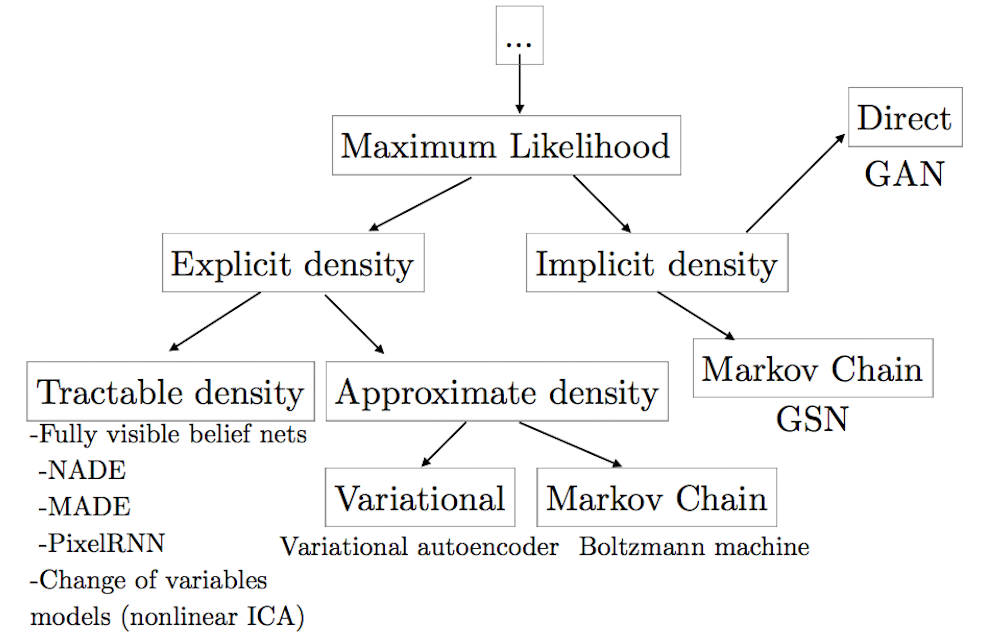
\includegraphics[width=0.8\textwidth]{./img/1.png}
\caption{生成模型分类}
\label{fig:taxonomy}
\end{figure}
在GAN发明人,Ian Goodfellow在NIPS2016的讲稿\cite{gan_tutorial}中,他曾将生成模型如图 \ref{fig:taxonomy}分类。可以看出GAN只是生产模型中新兴起的小分支。

本文主要介绍GAN的原理、进展及应用,但是也将在正式介绍之前适当介绍部分其他生成模型。

GAN的理论发展主要集中在损失函数上,比较有价值的几个进展是:
\begin{enumerate}
\item GAN,优化生成网络的JS散度
\item WGAN,优化生成网络的Wasserstein距离
\item LSGAN,机器学习确定损失函数
\end{enumerate}这些是本文的重点。

GAN的实践中总结出了很多技巧和模型,它们在图像生成任务中可以取得更好的效果。这样的工作最多,文章大部分的篇幅将围绕它们展开。

虽然GAN最初出现在图像领域,但是很多人将GAN应用于NLP、IR等其他领域,并取得了不错的效果。文章也将选择性地介绍几篇应用的文章。

文章的最后将介绍几篇强化学习的论文,在GAN的应用,特别是在序列数据生成方面,很多问题和强化学习中的问题是相似的,越来越多的任务使用了强化学习中的技巧。
\section{传统生成模型}
\subsection{Auto-Encoding Variational Bayes\cite{vae}}
Varitional AutoEncoder是一个传统的生成模型,它处理如下传统问题:

存在样本${x^{(i)}\in R^M}$,假设样本分布$P(x)$可以由如下两步生成:
\begin{itemize}

\item 生成隐变量$z\sim p_\theta(z)$,$z\in R^K$
\item 生成样本$x \sim p_\theta(x|z)$
\end{itemize}
同时由于x边缘似然难以积分(intractable),所有隐变量的后验概率$p_{\theta}(z|x) = \frac{p_\theta(x|z)p_\theta(z)}{p_\theta(x)}$是难以计算的。不能使用EM算法。

从
$D_{KL}(q(z|X)||p(z|X))=-\mathbb{E}_{z\sim q(z|X)}[\log\frac{p(z|X)}{q(z|X)}]$可以变形推出:
$$\log p(X)=D_{KL}(q(z|X)||p(z|X))+ L(p,q,X)$$
$$L(p,q,X)=-D_{KL}(q(z|X)||p(z))+\mathbb{E}_{z\sim q(z|X)}[\log p(X|z)]$$
由于KL散度大于0,L被称为variational lower bound。

我们的目标就是优化$q(z|X)$的参数$\phi$和$p(X|z)$的参数$\theta$,同时假设z的先验概率为$\mathcal{N}(0,I)$。根据q、p模型的不同,可以得到不同的VAE,文中给出的例子是二者均为多元高斯分布。

现在面临的另一个问题是,刚才的推断建立在针对单一样本X上。即使我们得到了一组最优的参数,可是它们只是条件概率的参数,对于其他样本来说仍然不适用。所以我们更希望得到的是$Q(X)\longrightarrow\phi、P(z) \longrightarrow \theta$这两个用神经网络去拟合。
\begin{figure}
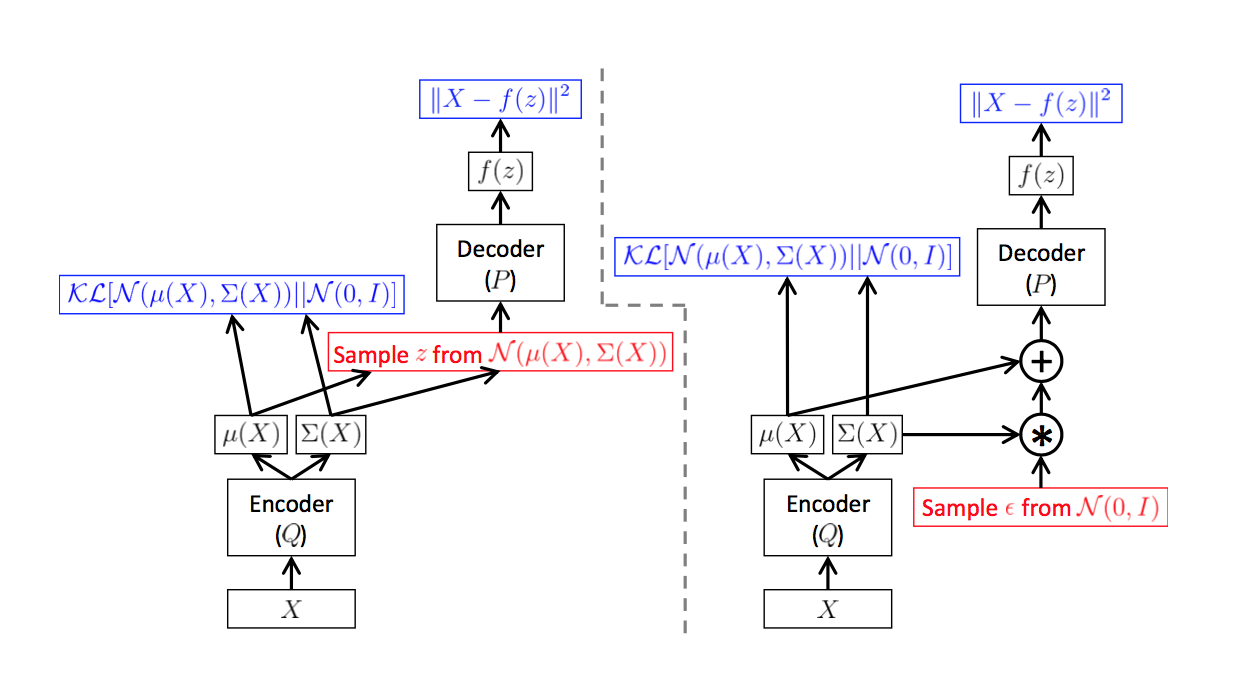
\includegraphics[width=\textwidth]{./img/2.png}
\caption{VAE}
\label{fig:vae}
\end{figure}
其实这里已经与假设有点不同了,假设的生成过程中$\theta$与$z$应该是无关的,而这里变成了z的函数。

但是网络上大部分的写法与论文差距更大——直接用神经网络拟合$p(X|z)$,可是X通常很高维且连续,神经网络不可能生成连续分布,于是将模型转化为隐式生成模型,并将sample得到的值同标准值的MSE作为loss的第二部分。

这种做法的原理未能查到任何出处。但是\citep{vae_toturial}以图\ref{fig:vae}的形式展示了这一做法。
\subsection{Generating Sequences With Recurrent Neural Networks\cite{DBLP:journals/corr/Graves13}}
这是通过RNN、LSTM等模型直接生成序列的方法,通过MLE进行训练。
\begin{figure}
\centering
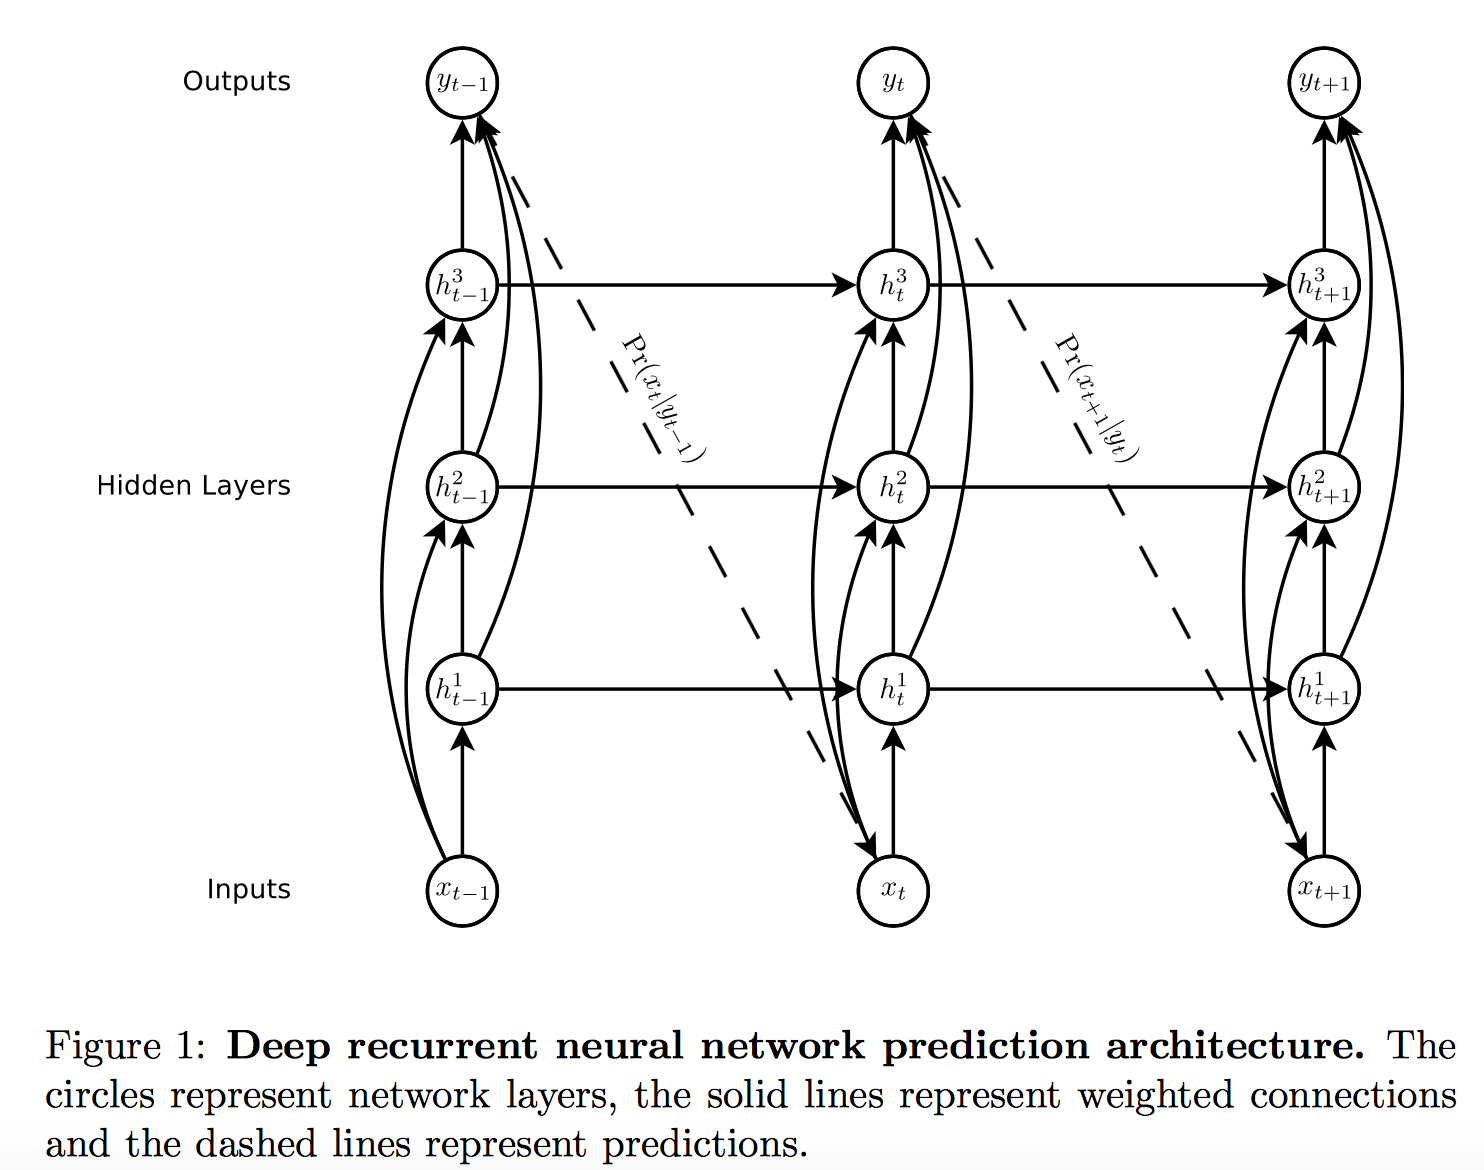
\includegraphics[width=0.8\textwidth]{./img/3.png}
\caption{RNN直接生成序列}
\label{fig:rnn}
\end{figure}
对于某个样本,$$loss = -\sum\limits_{t=1}^{T} log \ Pr(x_{t+1}|y_t)$$
具体做法是:
\begin{enumerate}
\item predict的时候$x_{-1}$为0,预测$y_0$,它是一个在字典上的条件概率分布,然后根据这个分布随机生成一个作为$x_0$输入到下一层,
\item train的时候使用上面的公式,每次输入数据中的元素,同时计算这个元素在模型中的生成概率,也就是$y_t$中的对应项。
\end{enumerate}
这里有个小trick,据说训练LSTM的时候梯度可能非常大,在LSTM的input处对梯度做截断。
\subsection{Photographic Image Synthesis with Cascaded Refinement Networks\cite{chen2017photographic}}
这是一篇与pix2pix的工作,针对其中的mask转化为真实图像的任务。文章使用了大量数据,没有采用GAN而是一种比较直接的卷积神经网络生成,取得了state-of-art的效果。

这说明监督学习中,如果有大量成对的数据,可能还是直接映射的方法比较好。文章输入mask图片,并且不断经过多个Module,每次分辨率长宽翻倍。每个Module分三层,输入上层的输出和相应大小的mask图片,输出一定channels(256)的图片。
\begin{figure}
\centering
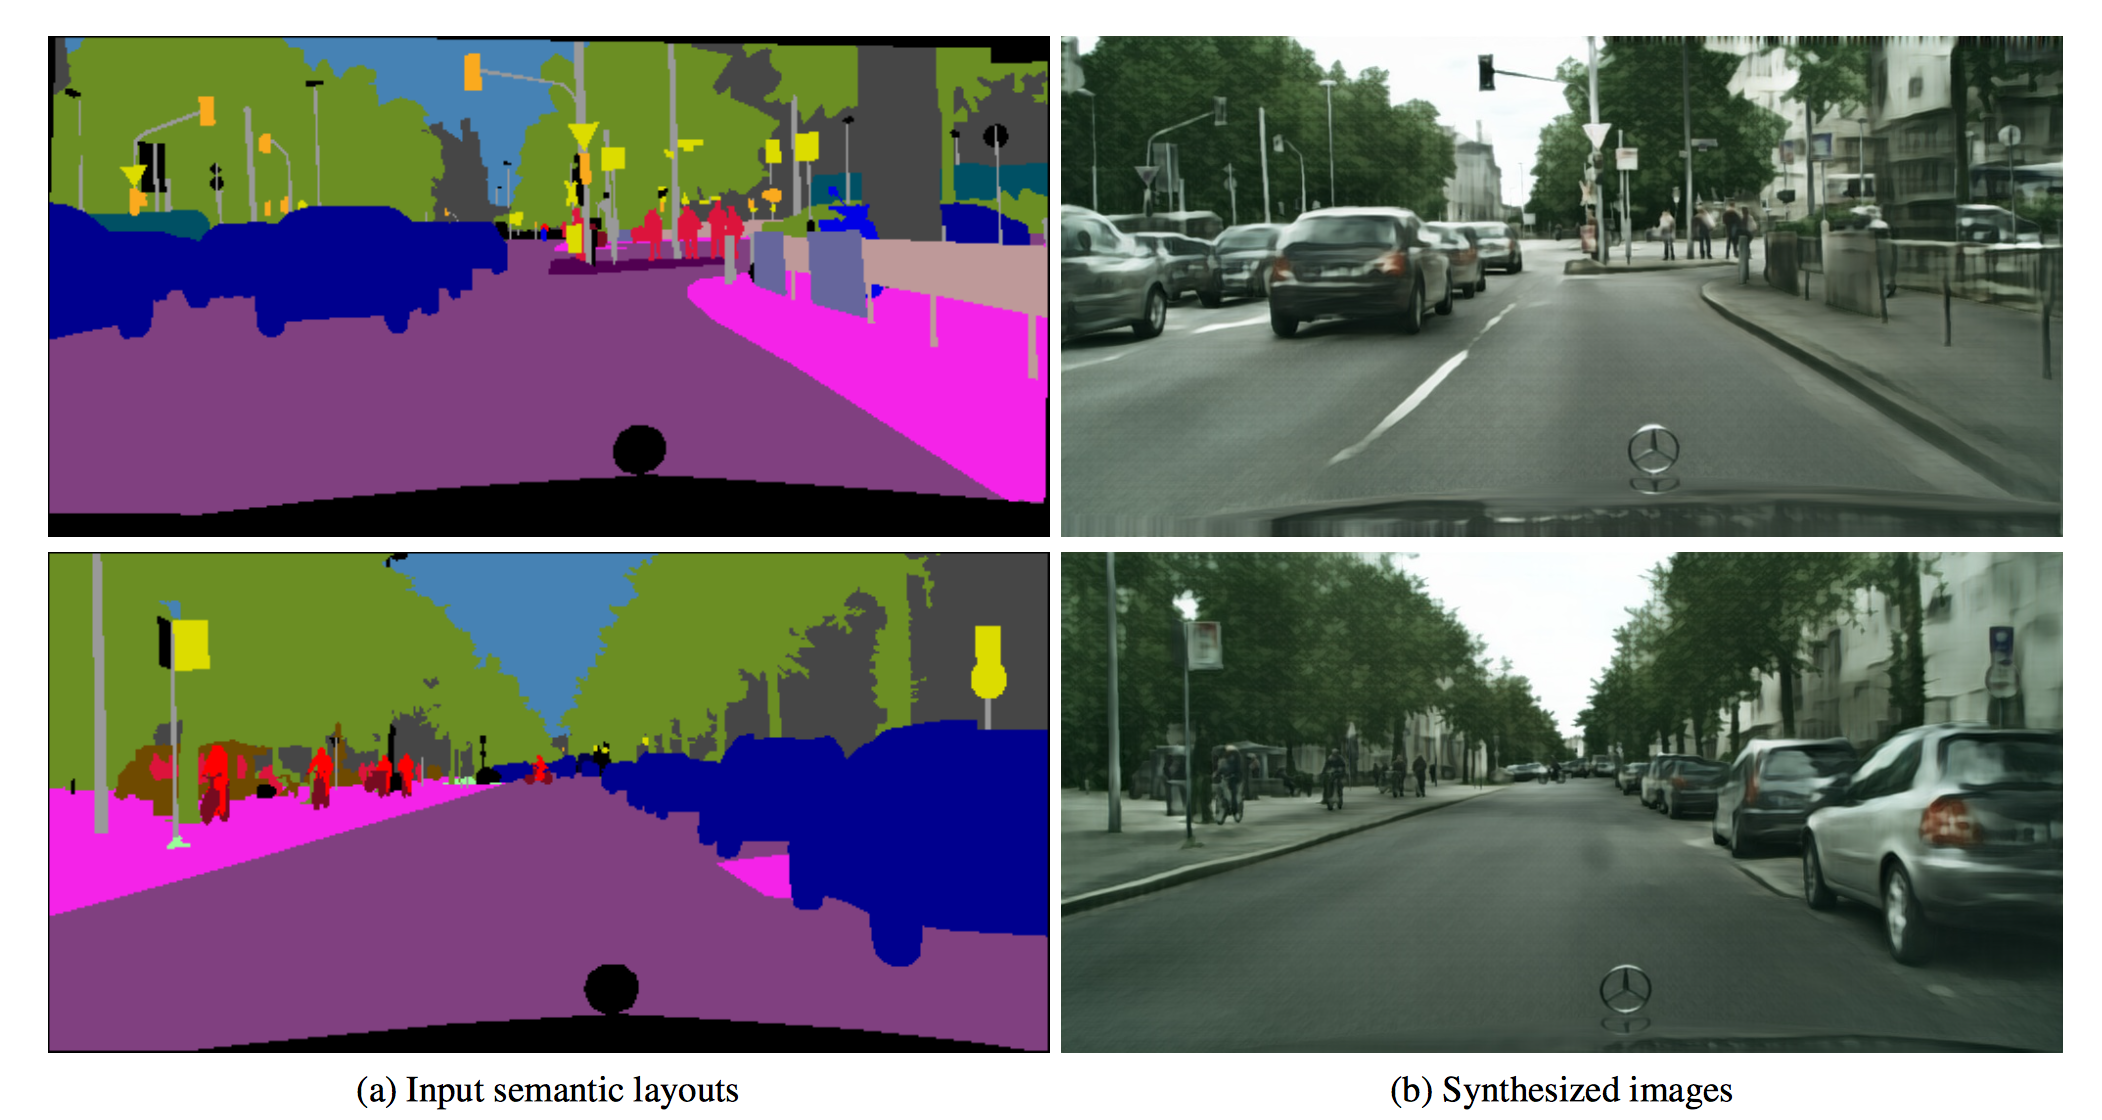
\includegraphics[width=0.8\textwidth]{./img/41.png}
\caption{photographic效果图}
\label{fig:41}
\end{figure}
效果图见\ref{fig:41}。注意最后的loss是生成图像、真实图像通过VGG网络各层之间的差距$\sum_l \lambda_l||\Phi_l(I)-\Phi(g_u(L,\theta))||_1$。
\section{GAN理论}
\subsection{原始GAN}
\subsubsection{Generative Adversarial Networks\cite{gan}}
如果我们抛开传统模型,重新考虑如何建立一个隐式的生成模型,最容易想到的是将高斯噪音通过神经网络,生成样本这样的模型。可是我们很快就发现没有办法训练它——贝叶斯方法很难用来训练神经网络参数,因为连$p(\mathcal{D}|\theta)$都无法确定。传统的神经网络通过梯度下降来优化损失函数,可是生成样本来自随机噪音并不能找到配对的真实样本。于是我们会去想将loss定义为与数据集中最近样本之间的距离(我并不确定这样效果如何,但找最近样本本身就挺费时的)等全局的方法,它们通常都不太优美。但是GoodFellow做到了,GAN应运而生。

GAN优化两个网络——生成网络G和判别网络D。生成网络通过噪音生成“假”样本,而判别网络判别样本的真假。
损失函数为
$$
\min_G \max_D V(D, G) = \mathbb{E}_{\bm{x} \sim p_{\text{data}}(\bm{x})}[\log D(\bm{x})] + \mathbb{E}_{\bm{z} \sim p_{\bm{z}}(\bm{z})}[\log (1 - D(G(\bm{z})))].
$$
\begin{algorithm}[ht]
\caption{\small Minibatch stochastic gradient descent training of generative adversarial nets.
The number of steps to apply to the discriminator, $k$, is a hyperparameter. We used $k=1$, the
least expensive option, in our experiments.
}
\begin{algorithmic}
\label{alg:AGF}
\FOR{number of training iterations}
  \FOR{$k$ steps}
    \STATE{$\bullet$ Sample minibatch of $m$ noise samples $\{ \bm{z}^{(1)}, \dots, \bm{z}^{(m)} \}$ from noise prior $p_g(\bm{z})$.}
    \STATE{$\bullet$ Sample minibatch of $m$ examples $\{ \bm{x}^{(1)}, \dots, \bm{x}^{(m)} \}$ from data generating distribution $p_\text{data}(\bm{x})$.}
    \STATE{$\bullet$ Update the discriminator by ascending its stochastic gradient:
        \[
            \nabla_{\theta_d} \frac{1}{m} \sum_{i=1}^m \left[
            \log D\left(\bm{x}^{(i)}\right)
            + \log \left(1-D\left(G\left(\bm{z}^{(i)}\right)\right)\right)
            \right].
        \]}
    %parameters $\theta_d$ of discriminator $D$
   %in the direction of the stochastic gradient of the binomial cross-entropy
   %for $D$ predicting whether its argument comes from $p_\text{data}(\bm{x})$ (target = 1, input = $\bm{x}$) or
   %$P_g$ (target = 0, input = $G(\bm{z})$), i.e., towards minimizing
   % \mbox{$-\log D(\bm{x}) - \log(1 - D(G(\bm{z})))$}.}
   \ENDFOR
  \STATE{$\bullet$ Sample minibatch of $m$ noise samples $\{ \bm{z}^{(1)}, \dots, \bm{z}^{(m)} \}$ from noise prior $p_g(\bm{z})$.}
    \STATE{$\bullet$ Update the generator by descending its stochastic gradient:
        \[
            \nabla_{\theta_g} \frac{1}{m} \sum_{i=1}^m
            \log \left(1-D\left(G\left(\bm{z}^{(i)}\right)\right)\right)
            .
        \]}
  \ENDFOR
  \\The gradient-based updates can use any standard gradient-based learning rule. We used momentum in our experiments.
\end{algorithmic}
\end{algorithm}
首先看从整个取值空间来看,
\begin{align}
V(G, D) =& \int_{\bm{x}} p_\text{data}(\bm{x}) \log(D(\bm{x})) dx + \int_z p_{\bm{z}}(\bm{z}) \log(1 - D(g(\bm{z}))) dz \nonumber \\
		=& \int_{\bm{x}} p_\text{data}(\bm{x}) \log(D(\bm{x})) + p_g(\bm{x}) \log(1 - D(\bm{x})) dx
\end{align}
如果我们充分优化D,对于每一个固定的x,被积项中D(x)都能取到$[0,1]$上的极大值$\frac{p_{data}}{p_{data} + p_g}$($a\log x+b \log (1-x)$求导)。
之后优化,\begin{align}
\label{eq:G-criterion}
 C(G) =& \max_D V(G,D) \nonumber \\
      =& \mathbb{E}_{\bm{x} \sim p_\text{data}}\left[\log \frac{p_\text{data}(\bm{x})}{P_\text{data}(\bm{x}) + p_g(\bm{x})}\right] + 
         \mathbb{E}_{\bm{x} \sim p_g}\left[\log \frac{p_g(\bm{x})}{p_\text{data}(\bm{x}) + p_g(\bm{x})}\right] \nonumber \\
      =& -\log(4) + KL \left(p_\text{data} \left \| \frac{p_\text{data} + p_g}{2} \right. \right) + KL \left(p_g \left \| \frac{p_\text{data} + p_g}{2} \right. \right) \nonumber \\
      =& - \log(4) + 2 \cdot JSD \left(p_\text{data} \left \| p_g \right. \right)\nonumber
\end{align}
于是Loss函数唯一最小值时有$p_g = p_{data}$。并且可以证明如果优化能在整个函数空间上进行,那么可以收敛。

\subsection{WGAN}
\subsubsection{Towards Principled Methods for Training Generative Adversarial Networks\cite{DBLP:journals/corr/ArjovskyB17}}
这
篇文章是WGAN前作,指出了GAN的问题所在。实际训练为什么要“平衡”生成和判别模型,而原文说直接将判别模型训练到最好就可以了。
原文指出D训练到最优时,$$D(x) = \frac{p_{data}(x)}{p_g(x) + p_{data}(x)}$$
此时对于生成模型的优化,$$L(D^*,g_\theta)=2JSD(\mathbb{P}_g||\mathbb{P}_{data})-2\log 2$$只需优化(梯度下降)这个JS散度。
但实际上,这个梯度下降难以进行。假设$p_{data}、p_{g}$重合度很低,此时发现JS散度是常数,没办法梯度下降。实际上他们都是高维空间(图像n*m)的低维流形,不重合概率很大。
原文提出的另一种改变G的loss则受梯度不稳定和mode collapse的困扰。

这篇文章给出的方法是给噪音退火,使得初值达到一个有不少重合的状态。
\begin{figure}
\centering
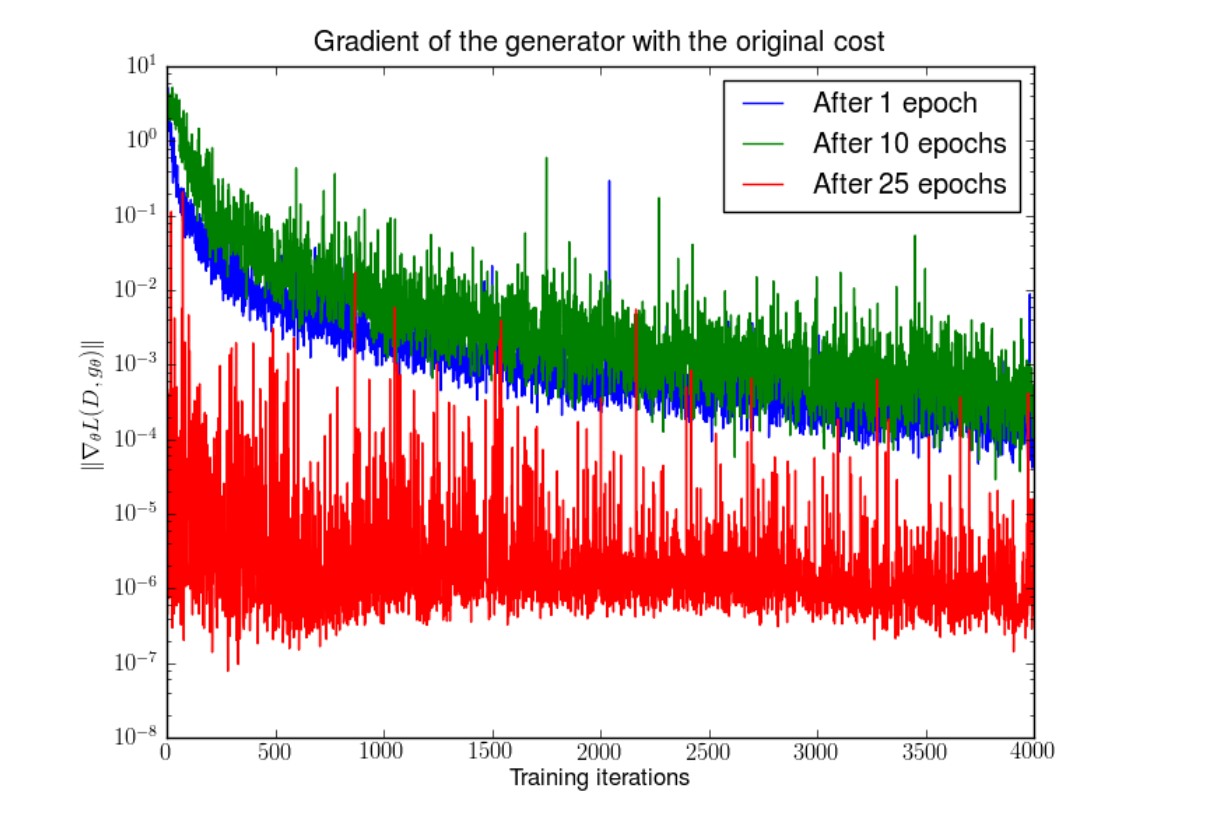
\includegraphics[width=0.8\textwidth]{./img/4.png}
\caption{训练时间与梯度}
\label{fig:4}
\end{figure}
\subsubsection{Wasserstein GAN\cite{DBLP:journals/corr/ArjovskyCB17}}
Wasserstein距离
$W(p_r,p_g)=\inf\limits_{\gamma\in \prod (p_r,p_g) }\mathbb{E}_{(x,y)\sim \gamma}[||x - y||]$
就是找一个分配方案,使得联合概率分布集中在对角线附近。一阶距就是Earth-Mover。
分布没有重叠的时候Wasserstein距离也有梯度。
有定理$$W(p_r,p_g) = \frac{1}{K}\sup\limits_{||f||_L\leq K}\mathbb{E}_{x\sim P_r}[f(x)]-\mathbb{E}_{x\sim P_g}[f(x)]$$
即对于所有满足Lipschitz条件的且Lipschitz常数小于K的函数中,期望差的上界。证明略。
用一个神经网络代替f的集合。为了满足Lipschitz常数小于K,强行将权值clip到一个规定的范围内。这样得到的值是Wasserstein距离的常数倍,梯度方向不变。

这个距离应该是G的loss,那么就用这个神经网络f代替D,使用样本充分训练使这个值极大后就代表了$p_g、p_r$之间的Wasserstein距离。那么最后实际更改的就只有:
\begin{itemize}

\item 判别器最后一层去掉sigmoid
\item 生成器和判别器的loss不取log
\item 每次更新判别器的参数之后把它们的绝对值截断到不超过一个固定常数c
\item 不要用基于动量的优化算法(包括momentum和Adam),推荐RMSProp,SGD也行
\end{itemize}
\begin{figure}
\centering
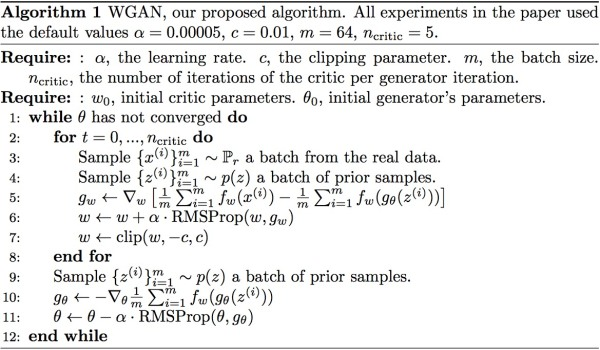
\includegraphics[width=0.8\textwidth]{./img/5.jpg}
\caption{WGAN算法描述}
\label{fig:5}
\end{figure}
\subsubsection{Improved Training of Wasserstein GANs\cite{DBLP:journals/corr/GulrajaniAADC17}}

weight clipping 有两个重要问题:\\
1. 倾向于最大最小值,可能减小网络表达能力\\
2. 容易梯度爆炸或消失\\
效果不太好。
于是不直接限制梯度,而是在后面加一个惩罚项。将判别器的目标改为
$$L = \mathbb{E}_{x\sim p_g}[D(x)]-\mathbb{E}_{x\sim p_r}[D(x)] + \lambda\mathbb{E}_{x\sim p_x}[(||\nabla_xD(x)||_2-1)^2], \lambda = 10$$
需要用到二阶梯度,可以用差分代替。
\begin{figure}
\centering
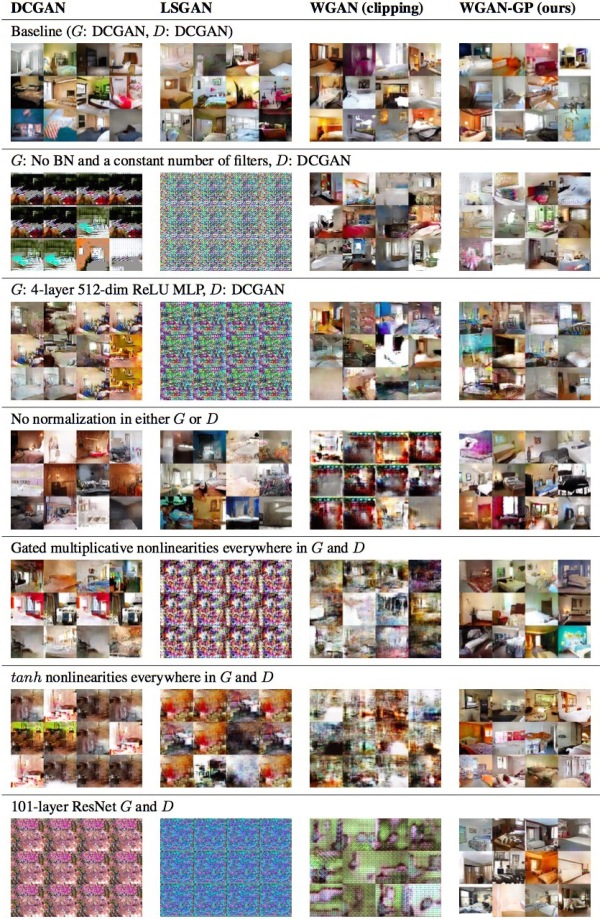
\includegraphics[width=0.8\textwidth]{./img/6.jpg}
\caption{效果比较}
\label{fig:6}
\end{figure}
\subsection{LS-GAN}

\subsubsection{Loss-Sensitive Generative Adversarial Networks on Lipschitz Densities\cite{DBLP:journals/corr/Qi17}}
GAN优化分布之间的JS散度,WGAN优化分布之间的Earth-Mover距离,而这篇文章通过Lipschitz假设认为这个loss-function可以通过真假样本间的距离之间学习,虽然我们没有成对的数据,但是由于Lipschitz条件,可以定性地认为真实分布集中在几个区域,那么我们可以将噪音分别映射到这些区域。
\begin{figure}
\centering
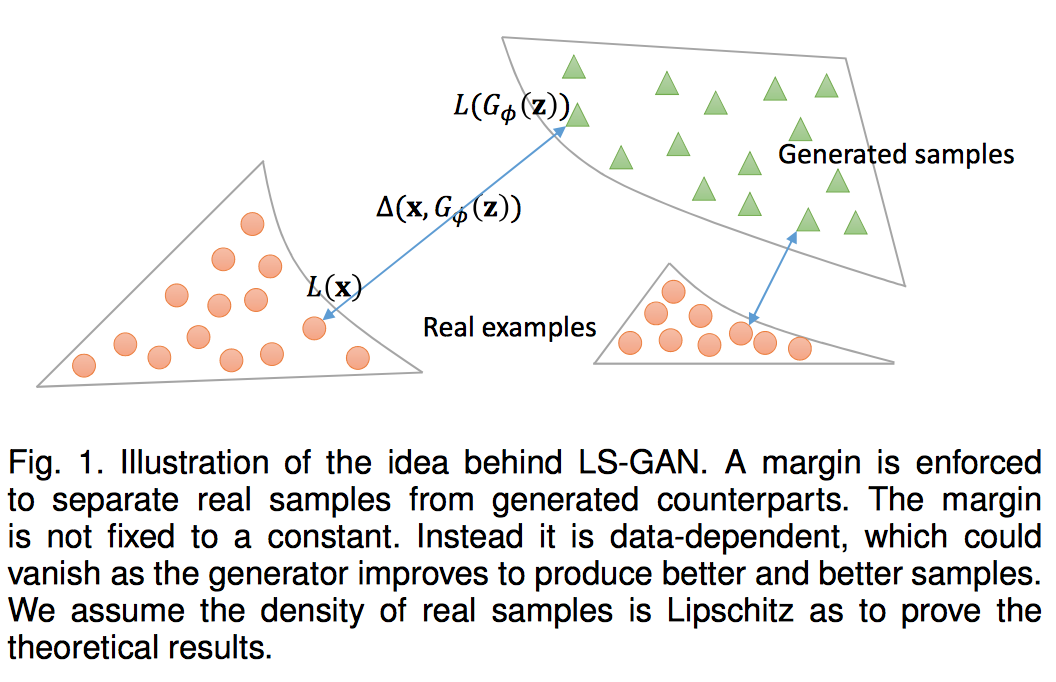
\includegraphics[width=0.8\textwidth]{./img/30.png}
\caption{LS-GAN图示}
\label{fig:30}
\end{figure}
我们定义$L_\theta$是一个对于真实样本输出较小值,对于假样本输出较大值的函数,同时满足限制
$$L_\theta(G(z)) - L_\theta(x) \geq \Delta(x, G(z))$$其中$\Delta$为样本距离比如一阶距。
所以我们可以轮流优化两个网络。

优化Loss function,$\mathbb{E}_{x\sim p_{data}}L_\theta(x)+\lambda\mathbb{E}_{x\sim p_{data},z\sim p_z}(\Delta(x, G(z)) - L_\theta(G(z)) + L_\theta(x))$
\begin{figure}
\centering
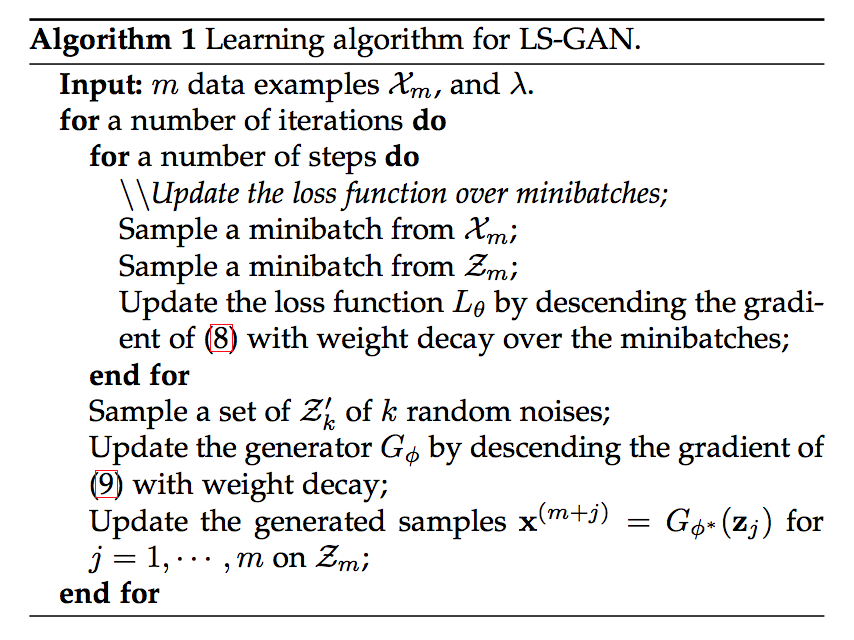
\includegraphics[width=0.8\textwidth]{./img/31.png}
\caption{LS-GAN算法}
\label{fig:31}
\end{figure}
优化G,$\mathbb{E}_{z\sim p_z}L_\theta(G(z))$。算法描述如\ref{fig:31}。
\subsection{基于能量函数的GAN的变体}
\subsubsection{Energy-based Generative Adversarial Network\cite{DBLP:journals/corr/ZhaoML16}}
\begin{figure}
\centering
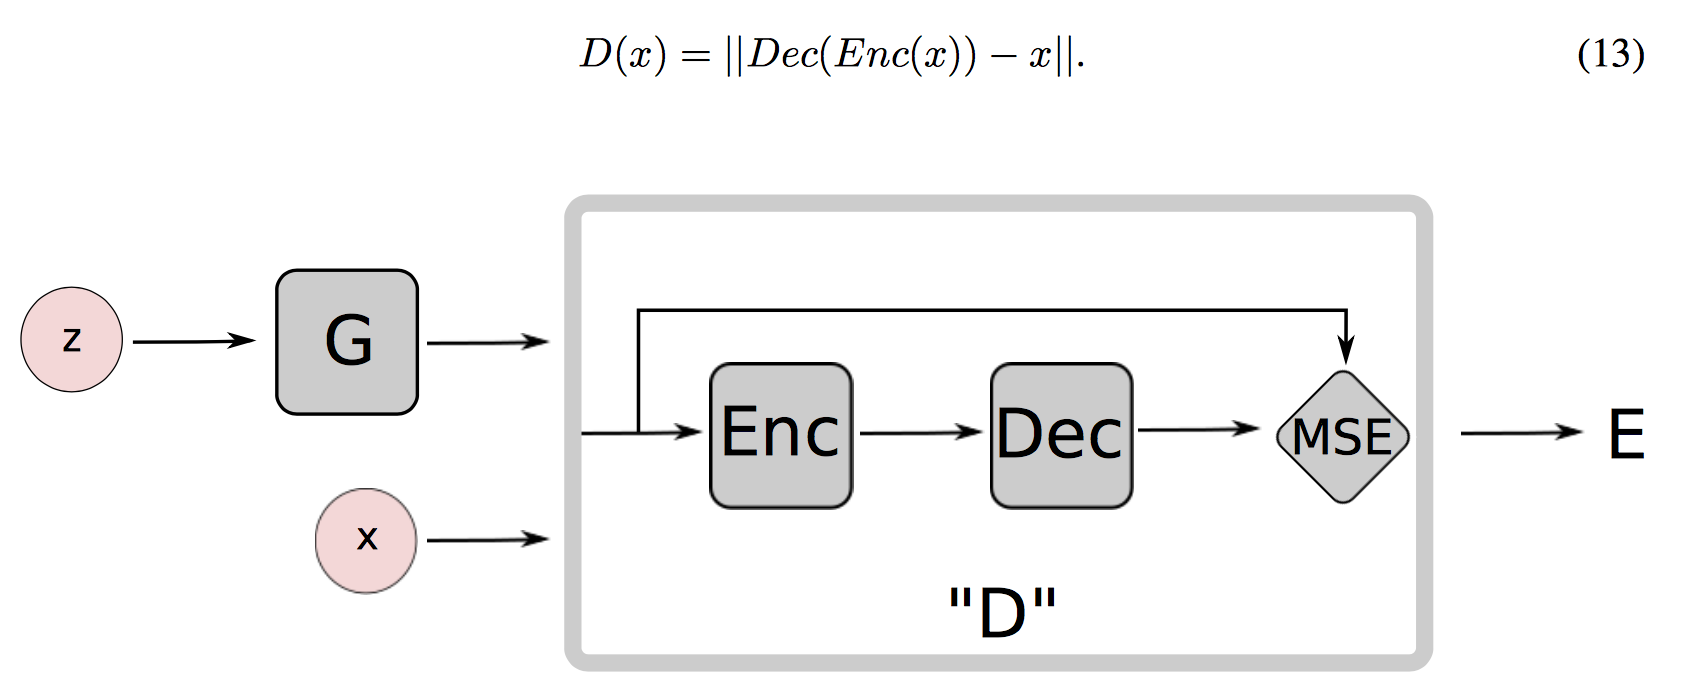
\includegraphics[width=0.8\textwidth]{./img/34.png}
\caption{EBGAN图解}
\label{fig:34}
\end{figure}
文章重定义了GAN的度量方法,假设存在一个能量函数,它在真实样本处接近于0,在假样本处接近于m。那么我们定义G,D的Loss为:
$$\mathcal{L}_D(x,z) = D(x) + max(m - D(G(z)),0)$$
$$\mathcal{L}_G(z) = D(G(z))$$
那么这个系统的Nash均衡点可以证明是$$p_g = p_{data}$$是得到。
定义loss-function为autoencoder的重构误差\ref{fig:34},认为这样做的好处是梯度来源提供的信息量比较大。
另外文章定义了一个pull-away term,让每个batch生成的有差别的一个loss项。
$$\frac{1}{N(N-1)}\sum\limits_i\sum\limits_{j \neq i}(\frac{S_i^TS_j}{||S_i||||S_j||})^2$$
S为encode出来的向量。
\subsubsection{BEGAN: Boundary Equilibrium Generative Adversarial Networks\cite{DBLP:journals/corr/BerthelotSM17}}
这篇文章是基于EBGAN的,首先修改了均衡的假设, 不再是真实样本为0,生成样本为m,而是满足一个接近1的倍数关系
\begin{figure}
\centering
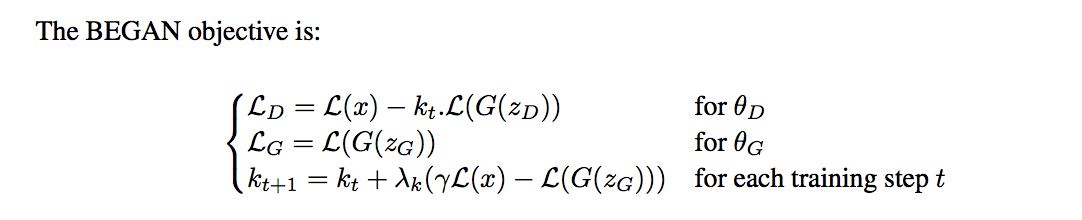
\includegraphics[width=0.8\textwidth]{./img/35.png}
\caption{BEGAN训练过程}
\label{fig:35}
\end{figure}
$$\gamma \mathcal{L}(x)=\mathcal{L}(G(z))$$
\begin{figure}
\centering
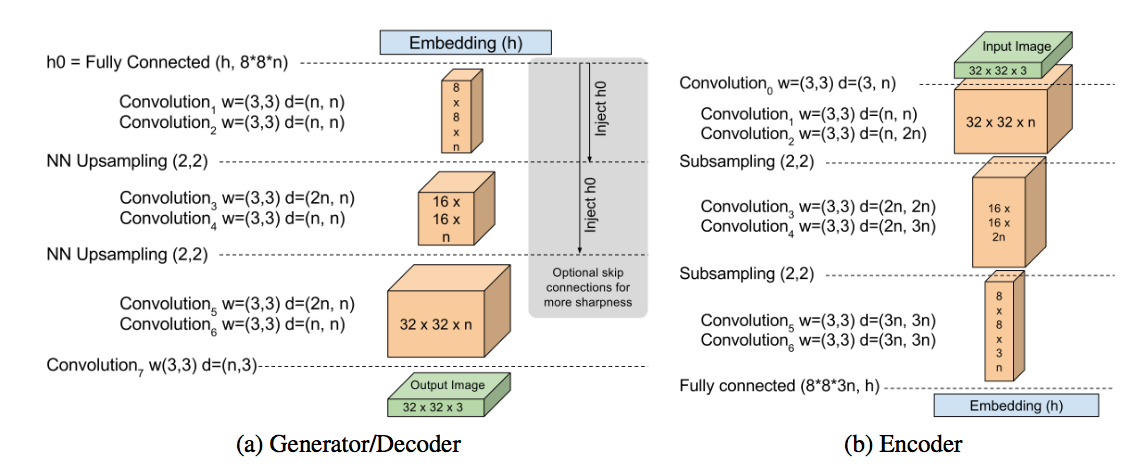
\includegraphics[width=0.8\textwidth]{./img/36.png}
\caption{EBGAN图解}
\label{fig:36}
\end{figure}
\subsection{GAN的问题}
\subsubsection{Do GANs actually learn the distributions? An empirical study\cite{DBLP:journals/corr/AroraZ17}}
作
者使用实验来说明GAN学出来的分布support size(离散分布中的非0点)不大,这是一个连续分布,用类(mode)代替。
根据生日悖论,如果我们能够随机抽一些看重复,可以估算出分布的support size。
\begin{figure}
\centering
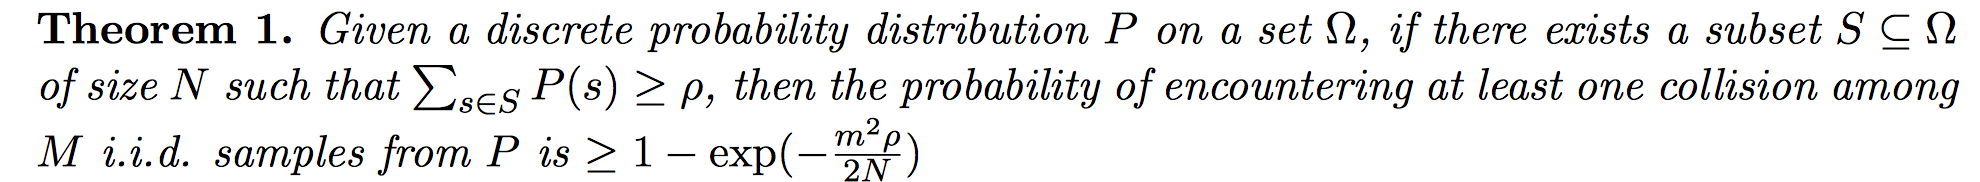
\includegraphics[width=\textwidth]{./img/7.png}
\label{fig:7}
\centering
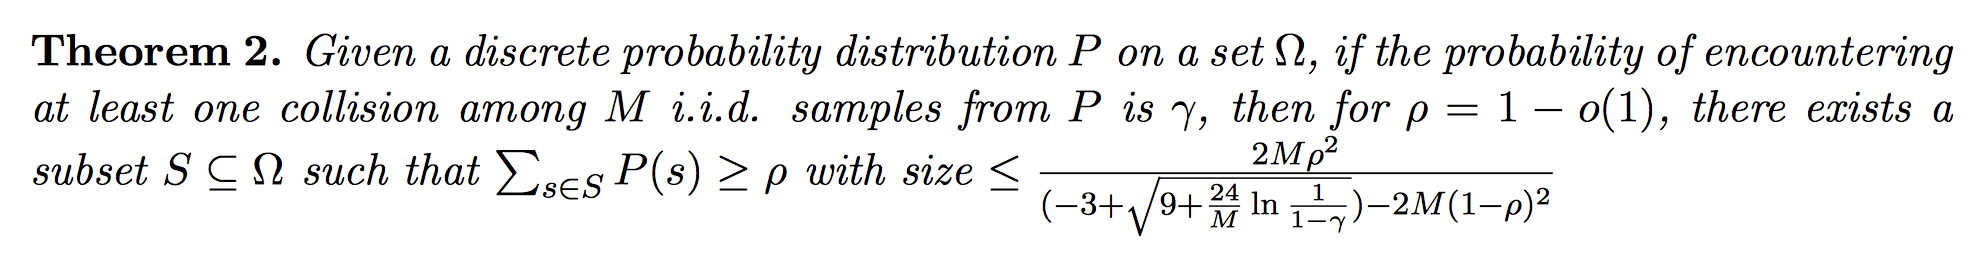
\includegraphics[width=\textwidth]{./img/8.png}
\caption{定理}
\label{fig:8}
\end{figure}

这样估计出了大部分概率构成的分布的support size的上界。实验证明学得的分布的support size远小于应有的数据集的support size。
证明了mode collapse的严重程度。
\section{GAN实践}
\subsection{高质量图片生成}
\subsubsection{Unsupervised Representation Learning with Deep Convolutional Generative Adversarial Networks\cite{DBLP:journals/corr/RadfordMC15}}
文章仅仅是将MLP用卷积神经网络实现了一下,但是通过细致的调参产生了很好的效果。\ref{fig:9}给出了一些设计的建议,\ref{fig:10}是最终使用的网络架构。
\begin{figure}
\centering
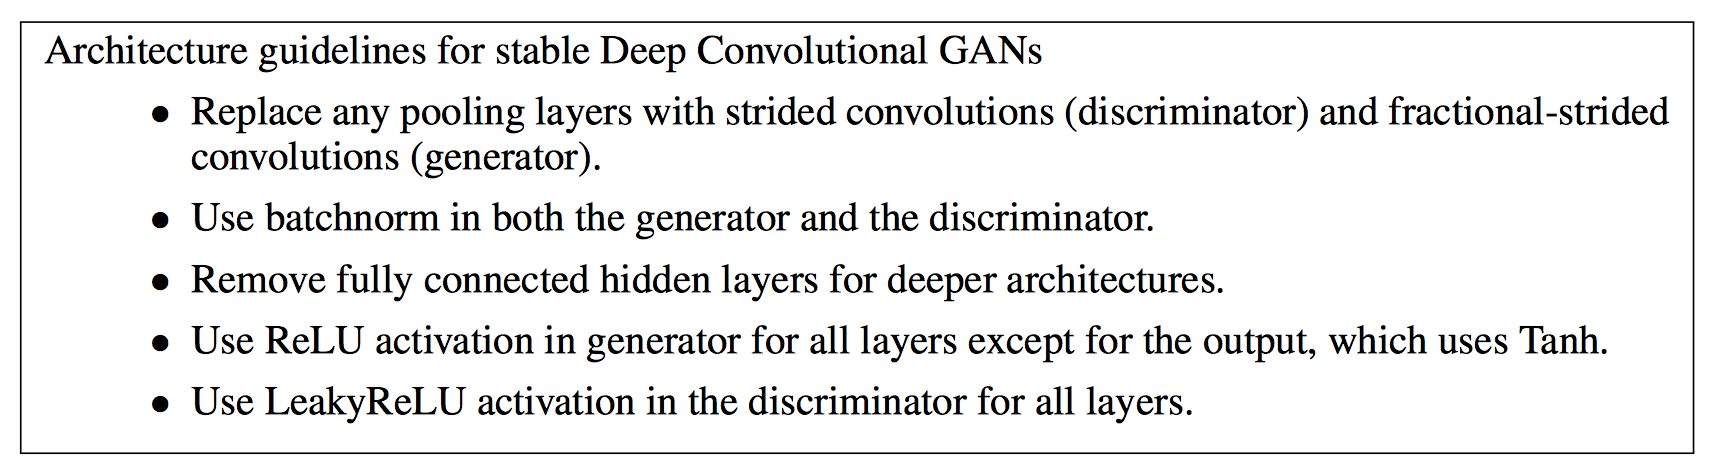
\includegraphics[width=\textwidth]{./img/9.png}
\caption{设计建议}
\label{fig:9}
\end{figure}
\begin{figure}
\centering
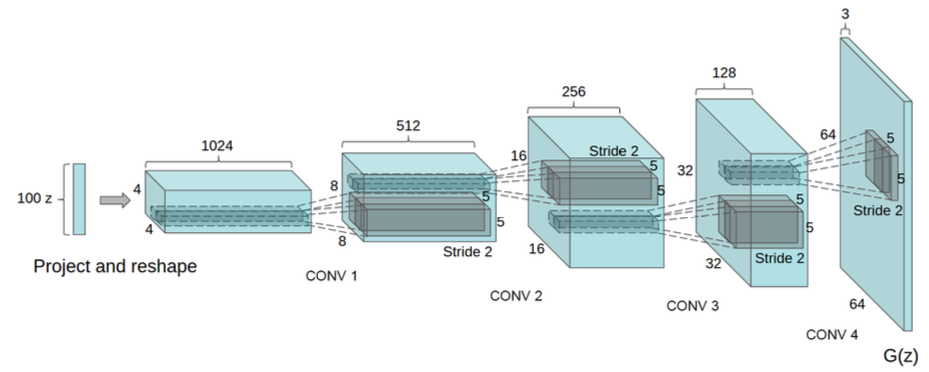
\includegraphics[width=\textwidth]{./img/10.png}
\caption{生成器架构}
\label{fig:10}
\end{figure}
\subsubsection{Deep Generative Image Models using a Laplacian Pyramid of Adversarial Networks\cite{DBLP:journals/corr/DentonCSF15}}
图像的laplacian金字塔在SIFT中用到过,但是这里似乎只用到了上下采样的层次,没有每个octave内部的分辨率变化。
于是我们训练多个GAN,直接生成最小的,然后conditional GAN的方法将upsampled的图像输进去生成差值。

\begin{figure}
\centering
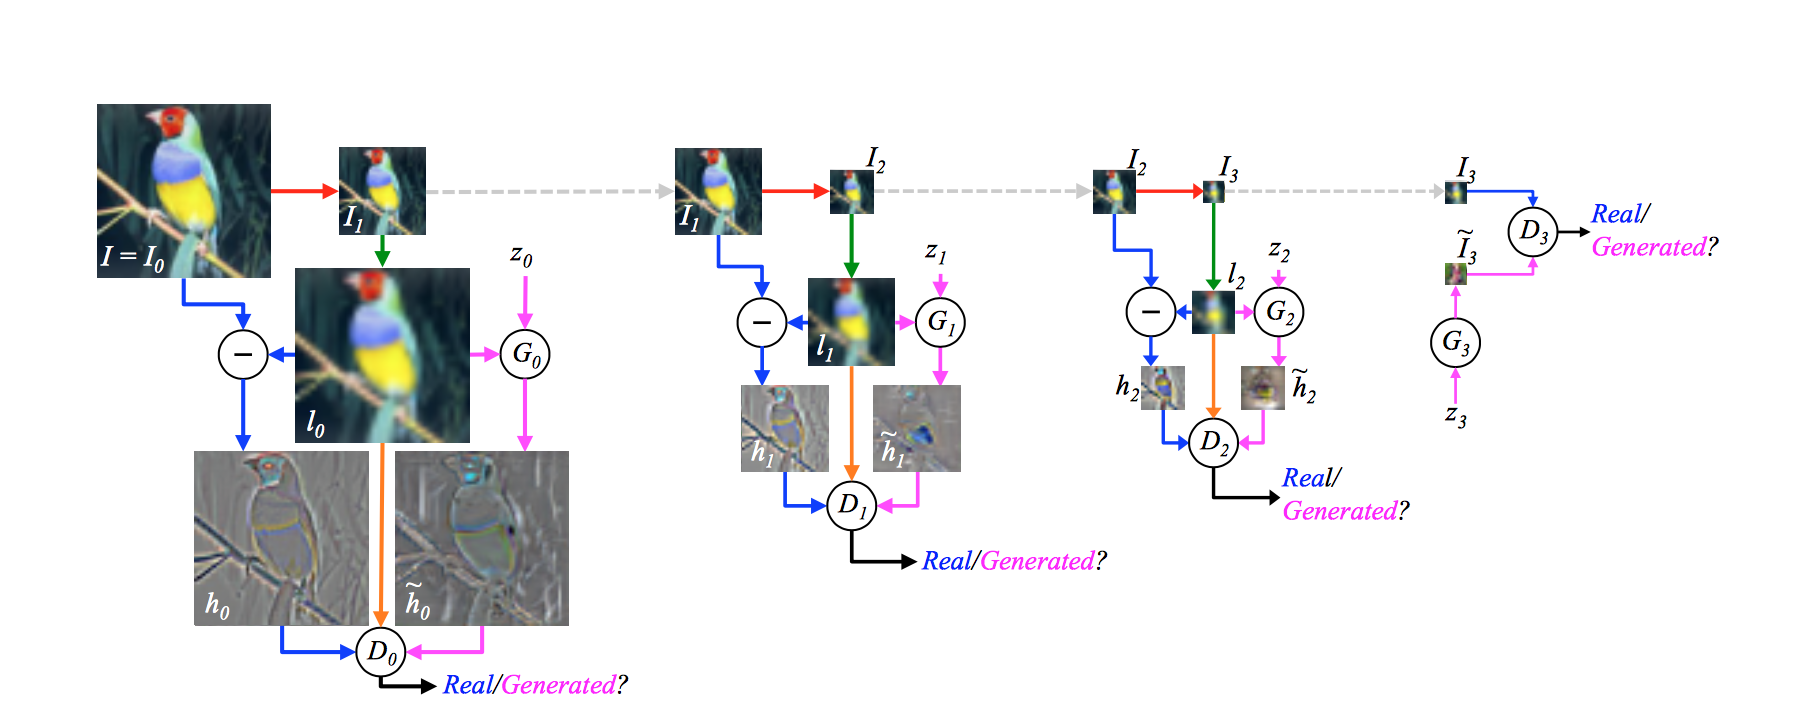
\includegraphics[width=\textwidth]{./img/15.png}
\caption{LAPGAN架构}
\label{fig:15}
\end{figure}解决“GAN直接生成图像一旦分辨率较大就出问题”。
\subsubsection{Generating Images Part by Part with Composite Generative Adversarial Networks\cite{DBLP:journals/corr/KwakZ16}}
想法是将图片生成问题分为多部分,比如背景、前景、装饰等……
使用一个RNN产生时序的输出,然后通过不同的G来生成不同的部分。
各部分通过alpha-blend融合在一起,就是将后一张图片中透明权重用前面生成的图片代替。
为了防止只有一个G起作用,增加了一个正则
$$|u - \sum C_{ijA}|-\sum (C_{ijA}-0.5)^2$$
其中u是一个自己定义的不透明度之和,防止前面都生成透明图像。后面的强迫透明度取0、1。
\begin{figure}
\centering
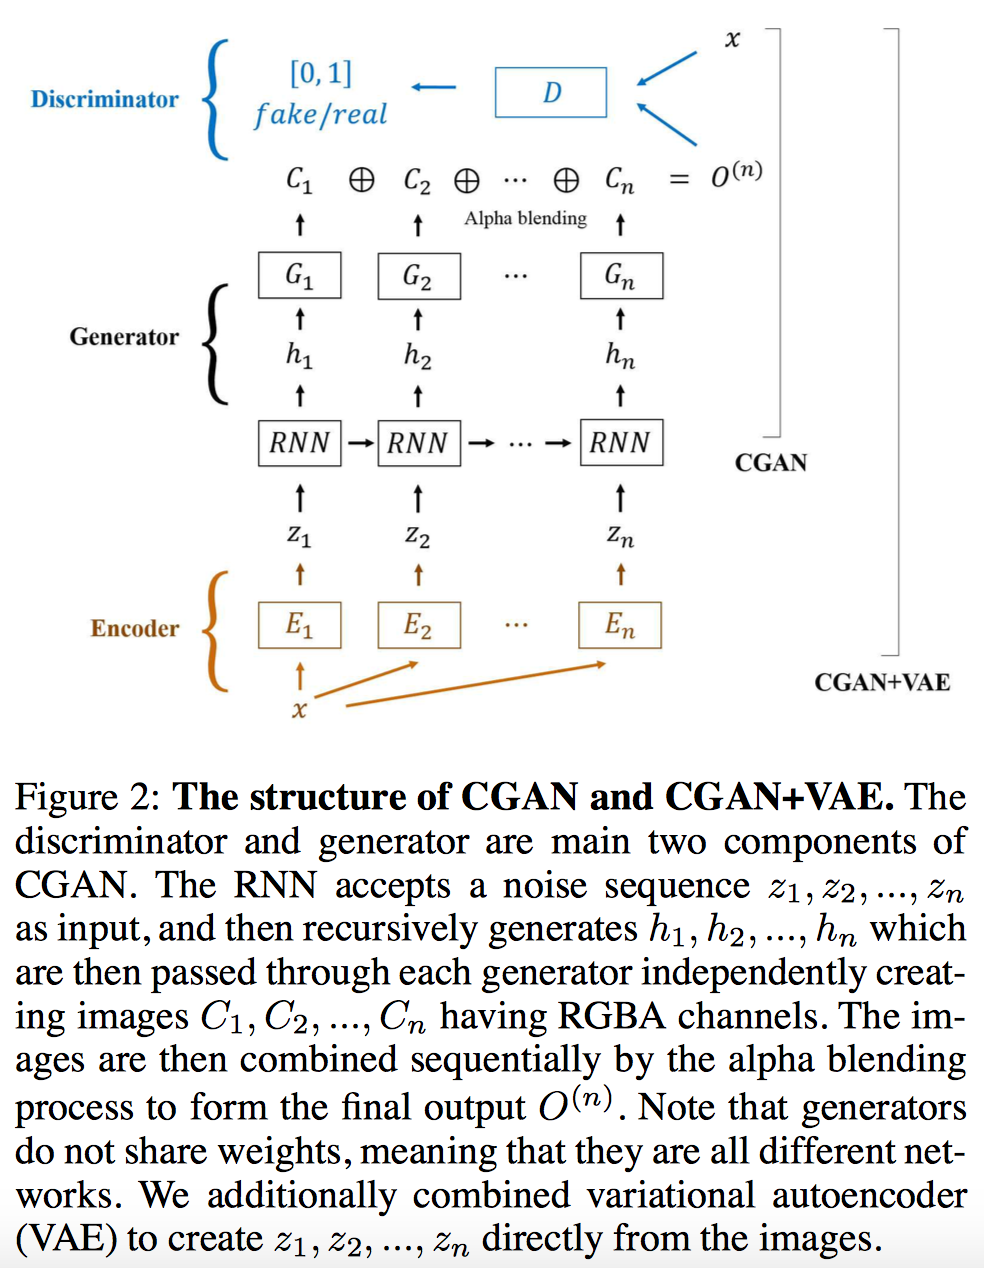
\includegraphics[width=0.8\textwidth]{./img/21.png}
\caption{Composite GAN架构}
\label{fig:21}
\end{figure}
\subsubsection{Generating images with recurrent adversarial networks\cite{gran}}
学习DRAW的生成方法,分部分生成,感觉结构与composite GAN很像。文章使用了一个很novel的度量方法,但是总之效果并没有很好。

文章将RNN每层换成了encoder-decoder结构,但是隐含层的状态并没有传入下一层。其中decoder生成图片,是一个DCGAN的生成器。

\begin{figure}
\centering
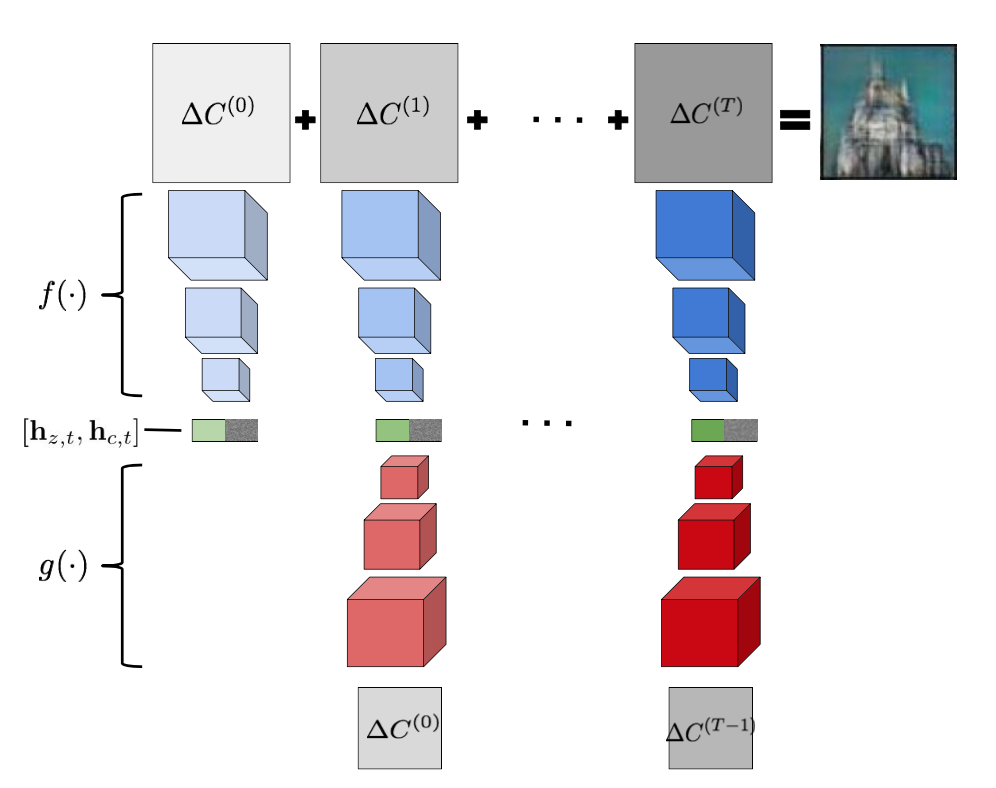
\includegraphics[width=0.8\textwidth]{./img/38.png}
\caption{GRAN架构}
\label{fig:38}
\end{figure}

\subsubsection{StackGAN: Text to Photo-realistic Image Synthesis with Stacked Generative Adversarial Networks\cite{DBLP:journals/corr/ZhangXLZHWM16}}
精心设计了两个GAN的架构,根据文本描述生成256*256的高质量图片。
\begin{figure}
\centering
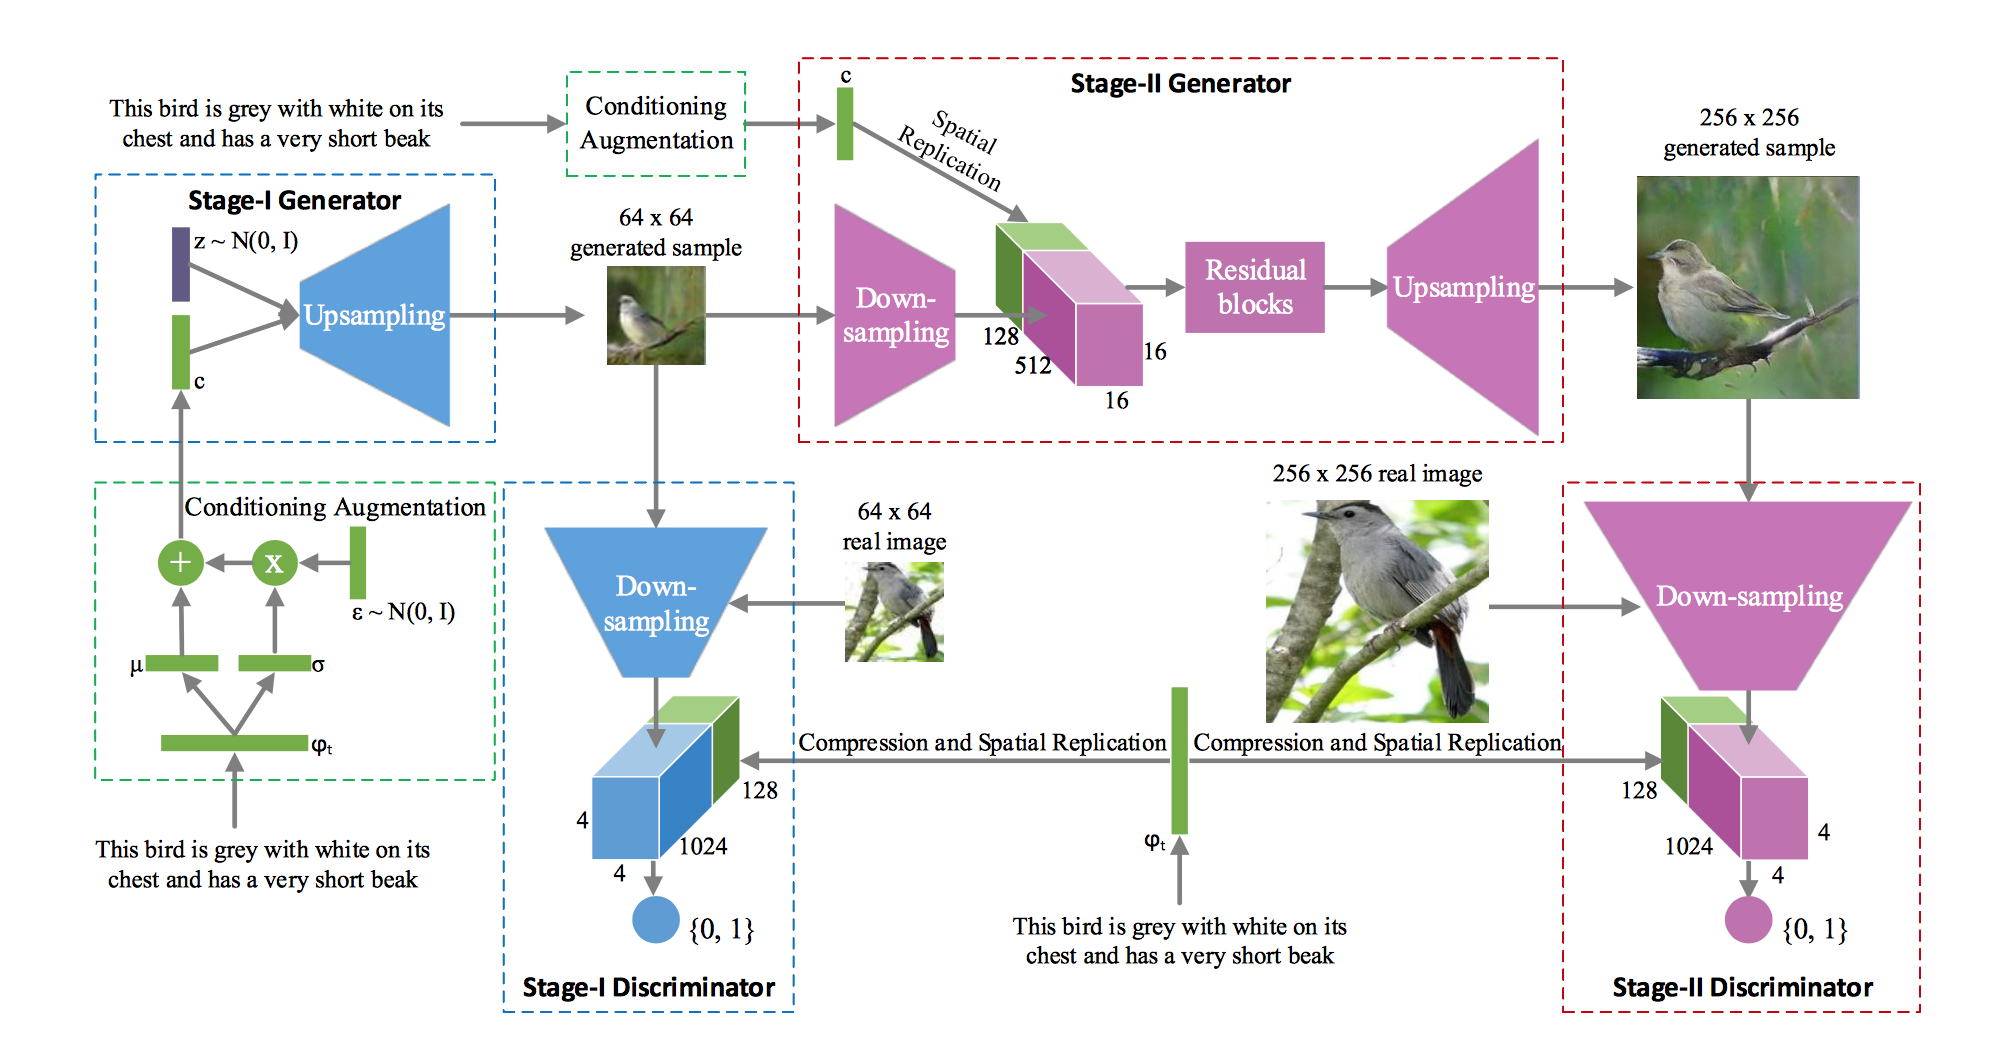
\includegraphics[width=\textwidth]{./img/16.png}
\caption{StackGAN架构}
\label{fig:16}
\end{figure}
值得注意的是,文本输入并没有直接使用embedding向量,作者认为向量过于稀疏效果不好,于是将向量通过两个神经网络生成一个N元高斯的均值向量和协方差矩阵,并加一项正则$$\lambda D_{KL}(\mathcal{N}(\mu(\phi_t),\Sigma(\phi_t))|| \mathcal{N} (0,I))$$使得这个分布尽量接近标准正态。
\subsection{pix2pix风格转换}
\subsubsection{Image-to-Image Translation with Conditional Adversarial Networks\cite{DBLP:journals/corr/IsolaZZE16}}
文章讨论如何将监督信息融入到GAN中,增加与真实转化图片的距离。给判别器和生成器的输入都增加转化前的原图。
\begin{figure}
\centering
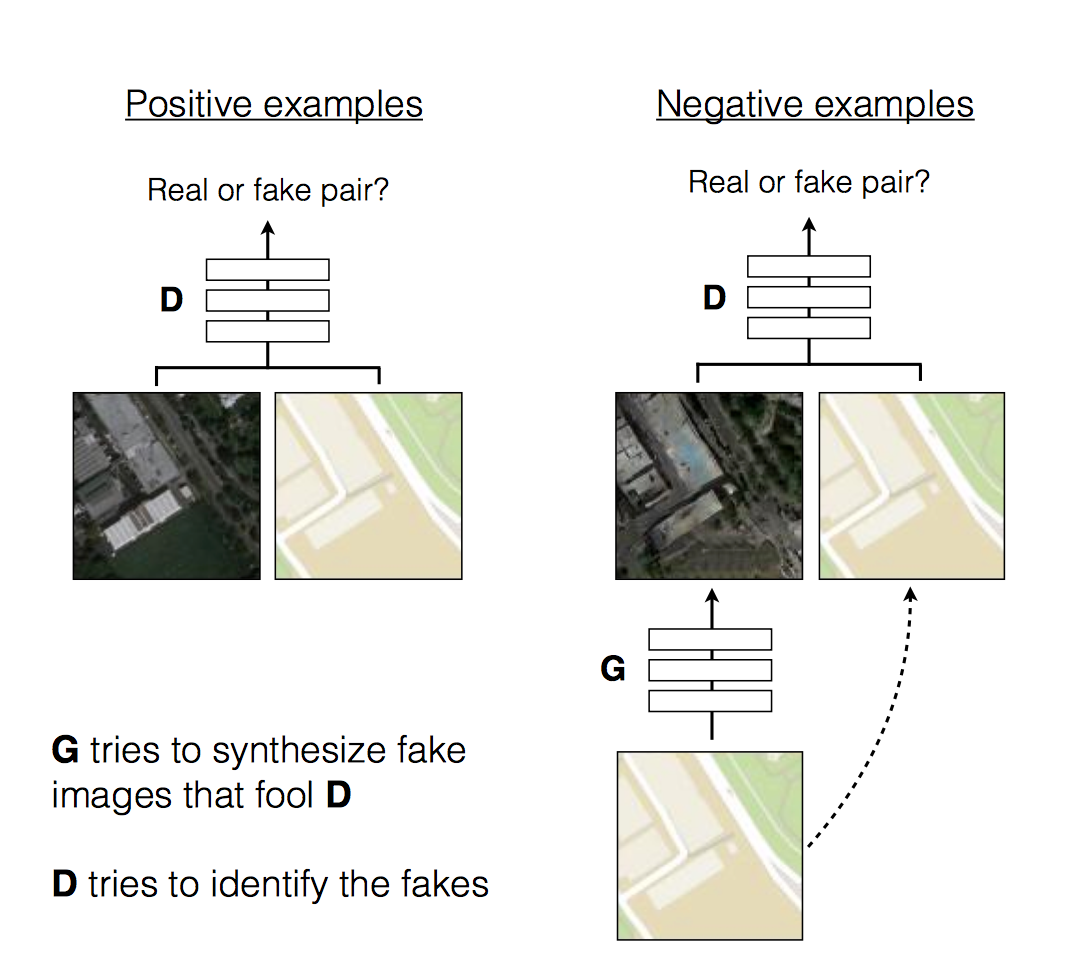
\includegraphics[width=0.8\textwidth]{./img/11.png}
\caption{Conditional GAN}
\label{fig:11}
\end{figure}
$$L_{L1}(G) = E_{x,y\sim p_{data}(x,y),z\sim p_z(z)}\left[||y-G(x,z)||_1\right]$$
$$L = L_{GAN}(G,D) + \lambda L_{L1}(G)$$
生成模型中使用了U-Net的结构,保证压缩信息的同时有原来的全部信息输入,这个与resNet有相同之处。

\subsubsection{Unsupervised Cross-Domain Image Generation\cite{DBLP:journals/corr/TaigmanPW16}}
\begin{figure}
\centering
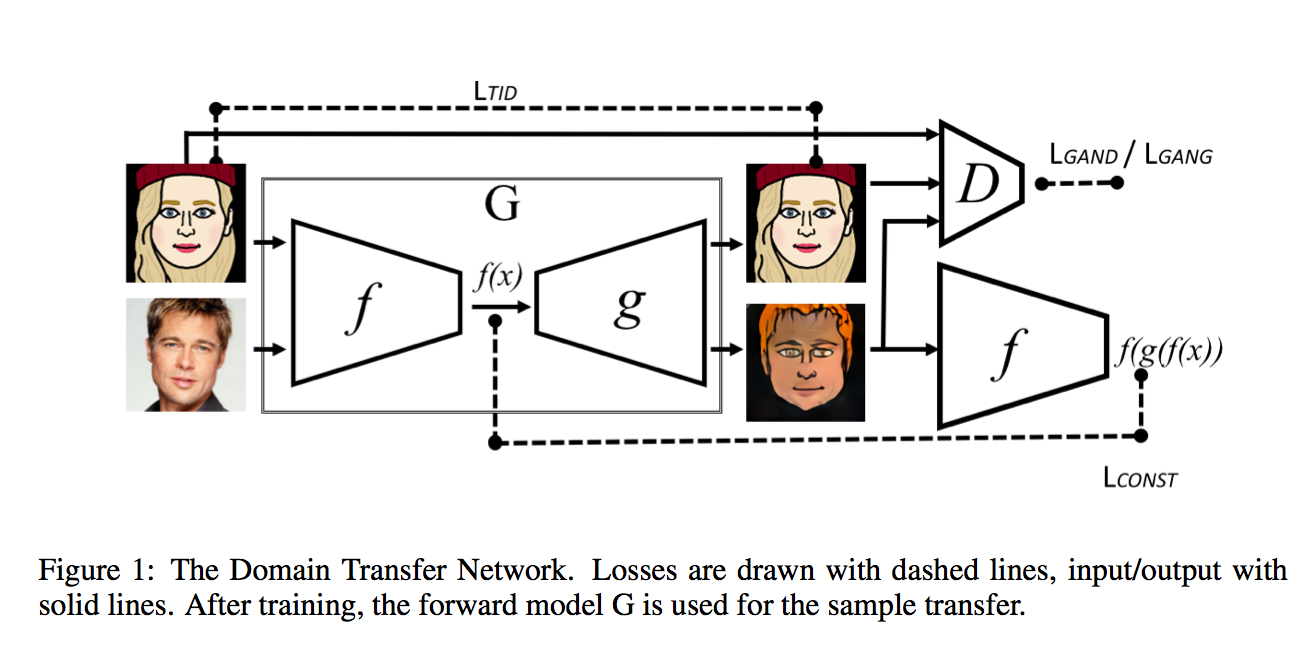
\includegraphics[width=\textwidth]{./img/12.png}
\caption{设计架构}
\label{fig:12}
\end{figure}
\begin{figure}
\centering
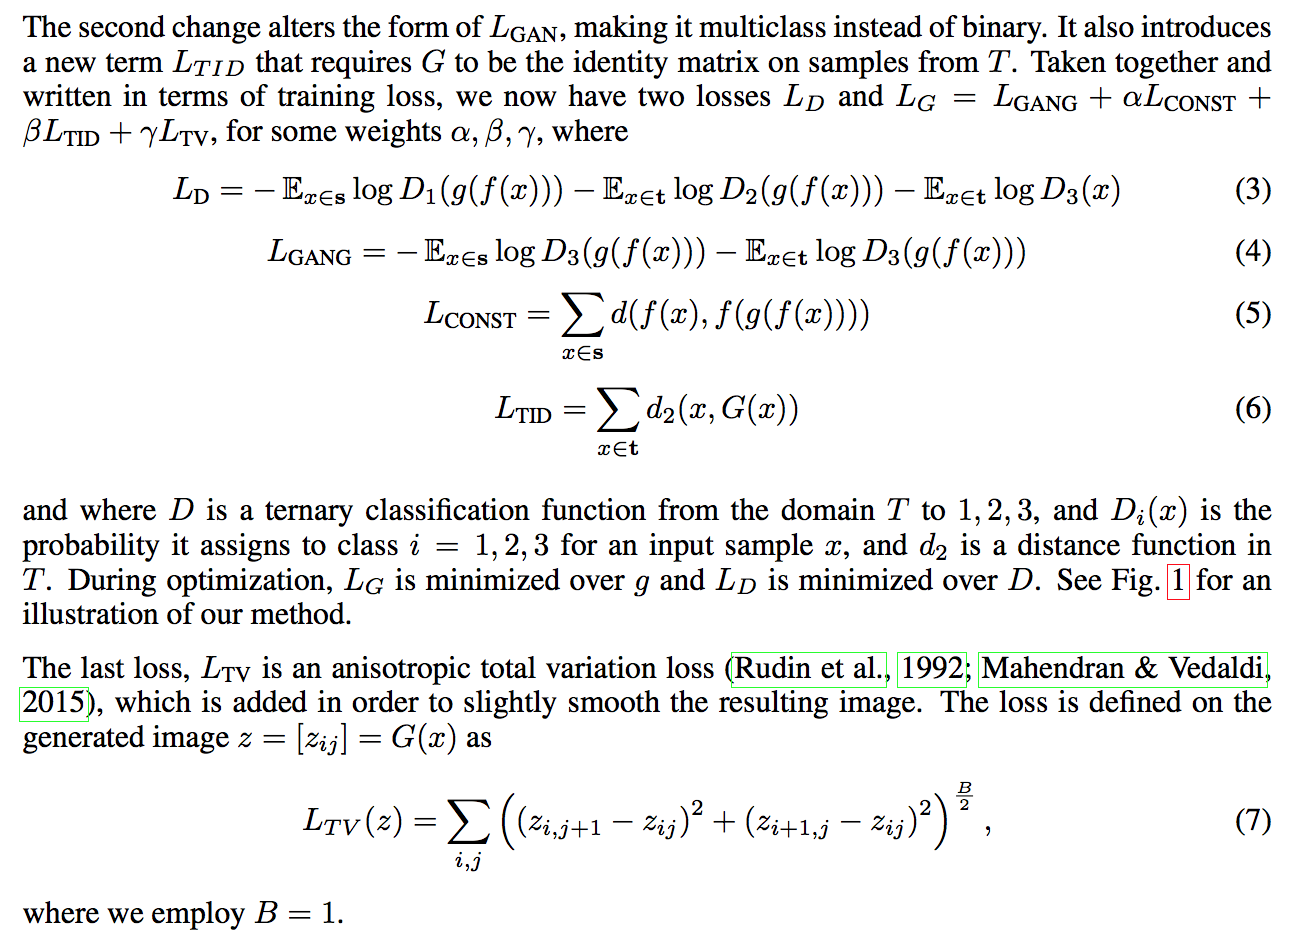
\includegraphics[width=\textwidth]{./img/13.png}
\caption{损失函数}
\label{fig:13}
\end{figure}
研究这样一个问题:存在两个不同的Domain S、T,学习G(s)->t。同时有一个定义在S并T上的函数f,使得经过G的变化之后f不变,f可能代表了整体架构之类的信息。
精心设计了复杂的网络\ref{fig:12},结合了auto-encoder(获得f)以及GAN。

共多项损失\ref{fig:13},但是lossTV最后没加。
\subsubsection{Unpaired Image-to-Image Translation using Cycle-Consistent Adversarial Networks\cite{DBLP:journals/corr/ZhuPIE17}}
还有两篇几乎同时发出的文章——Dual GAN、Disco GAN,做法相同。

\subparagraph{Question}
之前conditional GAN的一个应用是pix2pix,从一种类型的图片转化为相同框架的另一种类型的图片。但是需要配对的数据,很多时候我们并没有这样的数据,只有两类数据的样本若干。
\subparagraph{Method}
\begin{figure}
\centering
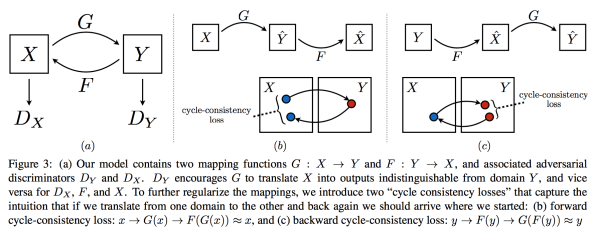
\includegraphics[width=\textwidth]{./img/18.png}
\caption{Cycle GAN原理}
\label{fig:18}
\end{figure}
通过重构误差。准确的说cycle consistency,这是一种历史悠久的技术了。具体见图\ref{fig:18}。
文章中完全取消了conditional GAN的随机性(反正也没什么用)。
$$L_{GAN}(G,D_Y,X,Y)=\mathbb{E}_{y\sim p_{data}(y)}[\log D_Y(y)]+\mathbb{E}_{x\sim p_{data}(x)}[\log D_Y(G(x))]$$
$$L_{cyc}(G,F)=\mathbb{E}_{x\sim p_{data}(x)}[||F(G(x))-x||_1]+\mathbb{E}_{y\sim p_{data}(y)}[||G(F(y))-y||_1]$$
实际将log换成平方效果更好。

仍然是对于style变化有用,对于有geometry变化的东西效果不好,如dog->cat。
\subsubsection{One-Sided Unsupervised Domain Mapping\cite{DBLP:journals/corr/BenaimW17}}
这
是一篇改进Cycle效果的文章。
将原来的cycle只保留一半,然后加一项正则。
$$L_{distance}(G_{AB},\hat{p_A})=\mathbb{E}_{x_i,x_j\sim \hat{p_A}}|\frac{1}{\sigma_A}(||x_i-x_j||_1-\mu_A)-\frac{1}{\sigma_B}(||G_AB(x_i)-G_AB(x_j)||_1-\mu_B)|$$
就是说原来domain的文章变换过去要归一化保距,这就更加强行限制了少出现mode collapse。
\begin{figure}
\centering
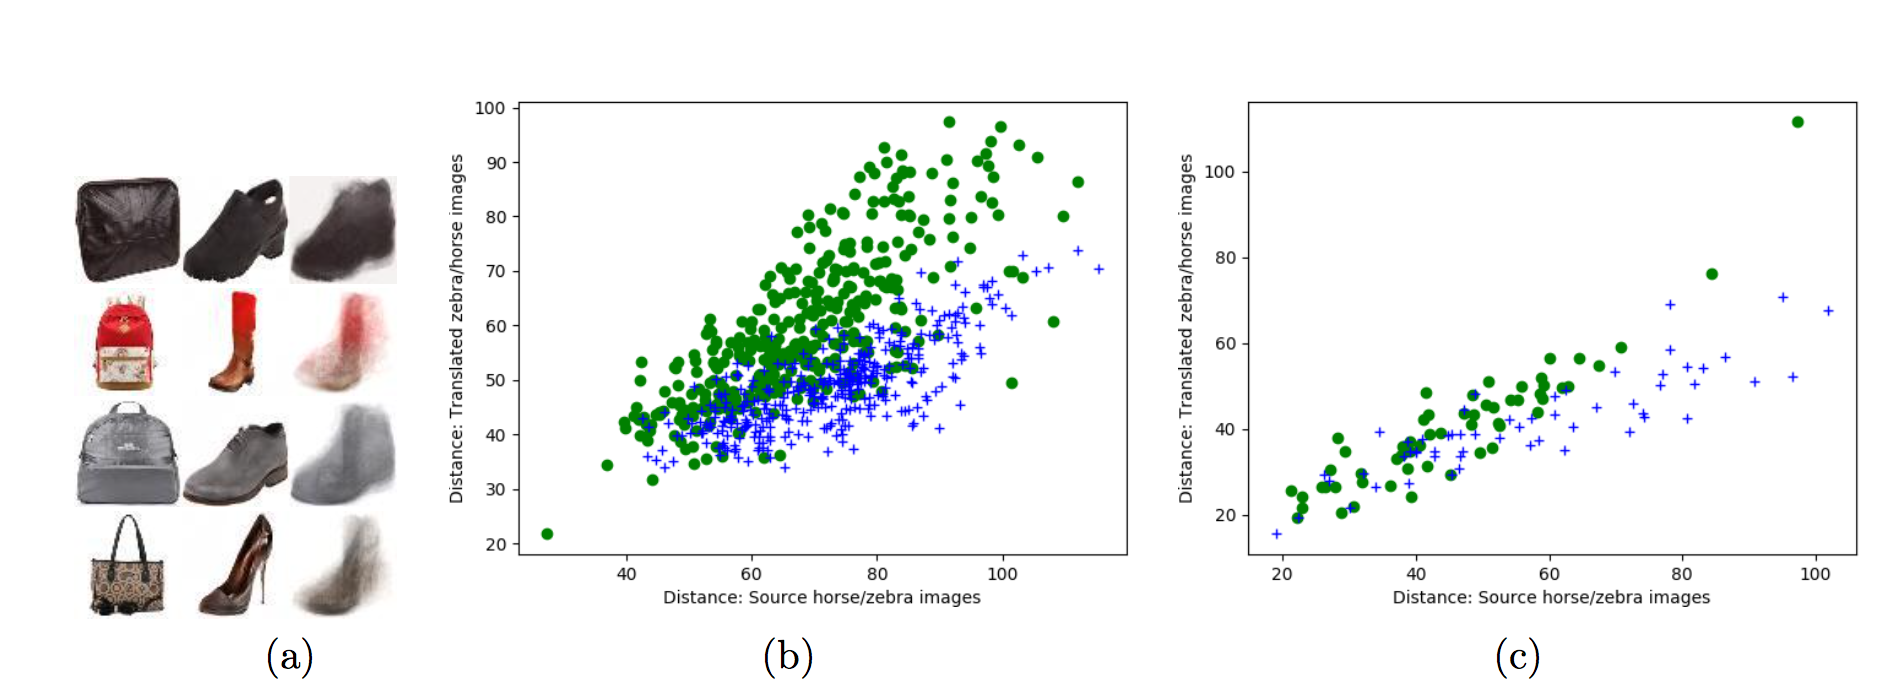
\includegraphics[width=\textwidth]{./img/19.png}
\caption{Distance GAN效果}
\label{fig:19}
\end{figure}
\subsubsection{Generative Semantic Manipulation with Contrasting GAN\cite{semantic_replace}}
\begin{figure}
\centering
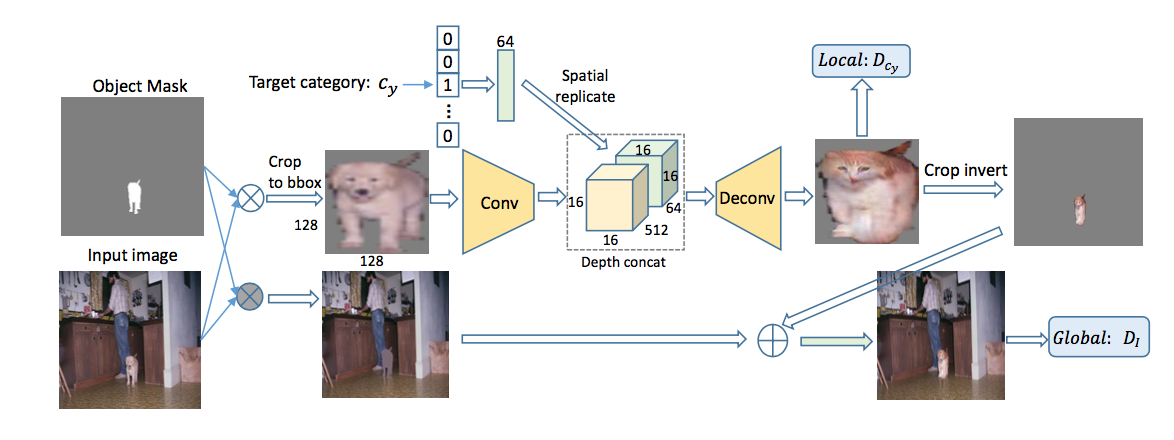
\includegraphics[width=\textwidth]{./img/37.png}
\caption{mask-conditional contrast-GAN}
\label{fig:37}\end{figure}
文章针对cycle GAN不能大幅改变物体的特点,提出用一个mask先找出需要替换的物体,然后用GAN生成另一类物体强行替换进去。\ref{fig:37}

GAN生成的时候基本是基于Cycle GAN,但是加入一项contrast loss。
$$Q(f_{y'},f_x,f_y)=-\log \frac{e^{-||f_{y'}-\overline{f_y}||}}
{e^{-||f_{y'}-\overline{f_y}||} + e^{-||f_{y'}-f_x||}}$$

\subsection{生成控制}
\subsubsection{Conditional Image Synthesis With Auxiliary Classifier GANs\cite{DBLP:journals/corr/OdenaOS16}}
利
用监督信息生成特定类图片。做法就是G输入噪音和类别信息,加入第二个D判别类别,这里类别判断都要最大化likelihood。
$$L = L_{GAN}(G,D_1) + \mathbb{E}_{x\sim c_i}[\log D_2(x)_i]$$
后一项包括真假两种情况,按照输入G时的c来定。
\begin{figure}
\centering
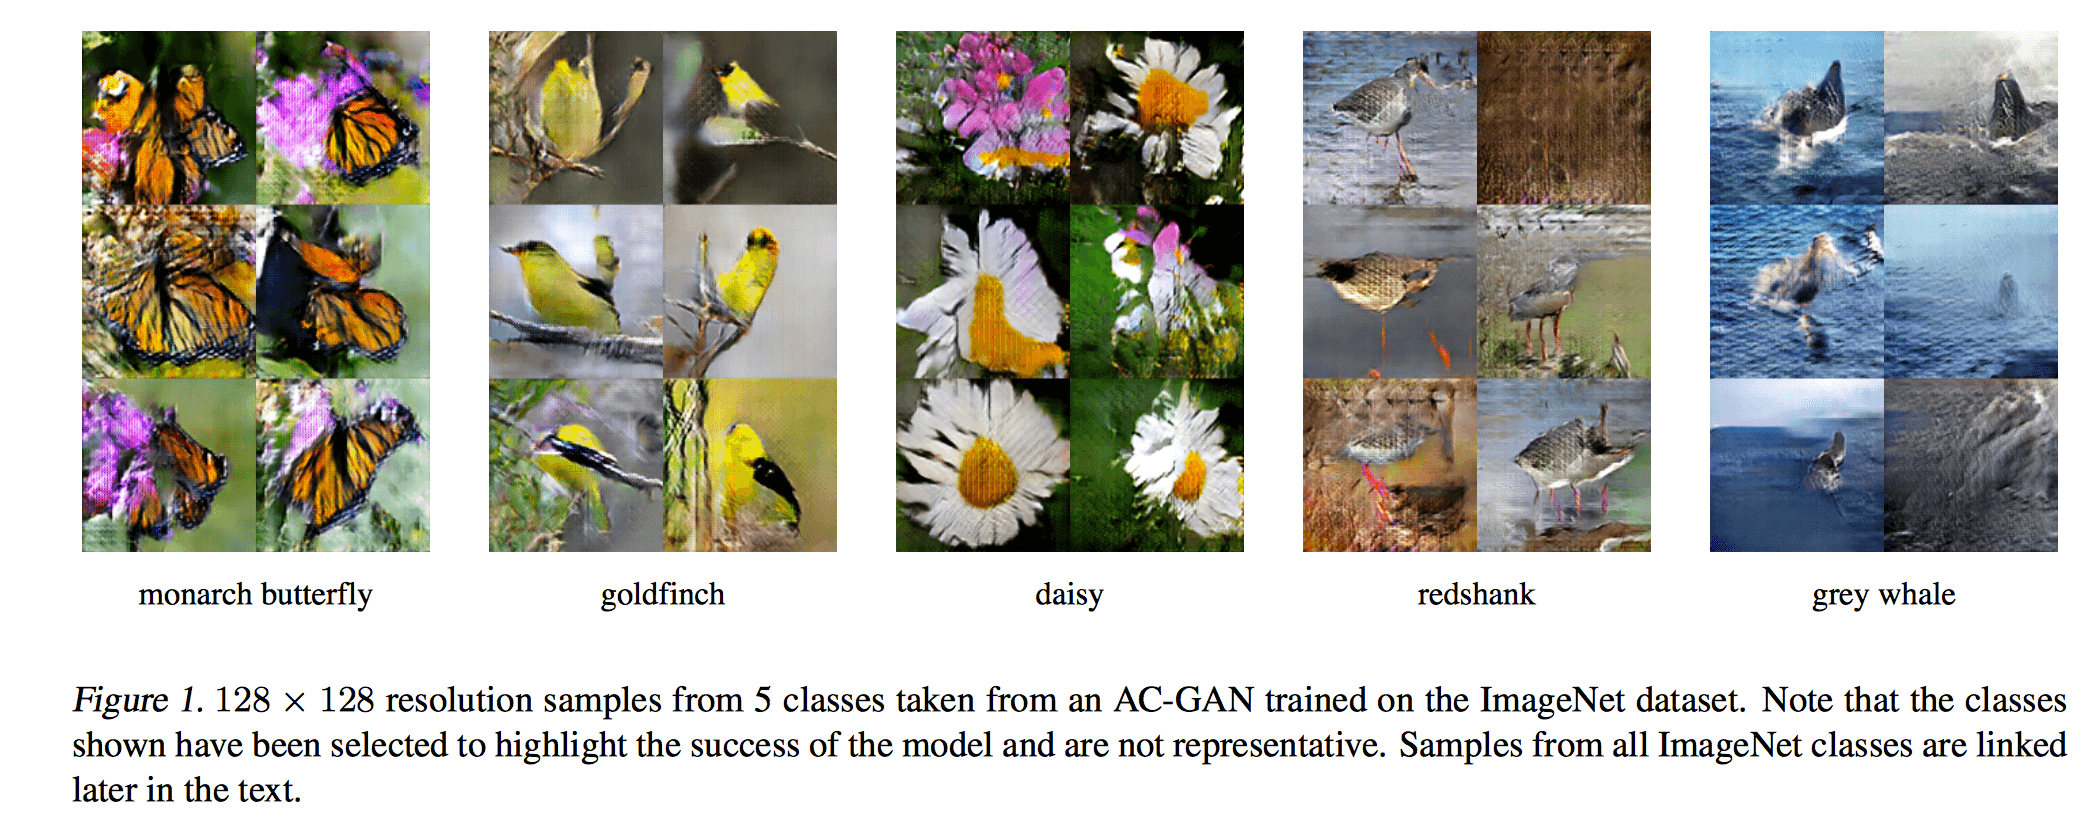
\includegraphics[width=\textwidth]{./img/14.png}
\caption{AC-GAN效果}
\label{fig:14}
\end{figure}
\subsubsection{InfoGAN: Interpretable Representation Learning by Information Maximizing Generative Adversarial Nets\cite{DBLP:journals/corr/ChenDHSSA16}}

 \subparagraph{Question}
G学习的是噪音分布到数据分布的映射,之前研究发现噪音向量有类似于word2vec的线性性质,但是具体想控制某个特征很难。希望能够让输入向量是disentangled representation的表示。
\subparagraph{Method}
\href{https://sleepychord.gitbooks.io/volume1/content/xin-xi-lun-ji-chu.html}{信息论概念} 
确定一部分控制输入c,加regularization,使得已知生成样本后,对输入c的互信息很大。由于c是我们控制的,优化G只能将多个差异较大的样本分配给不同的c,这样就可以显式控制了。
$$\min\limits_G\max\limits_D V_I(D,G)=V(D,G) - \lambda I(c;G(z,c))$$

由于不知道真实分布,更不知道条件分布,没办法计算互信息,可以通过自己构造的模型代替p,并且把条件概率改为c的先验概率。
$$I(c;G(z,c))\approx \mathbb{E}_{c\sim P(c), x\sim G(z,c)}[\log Q(c|x)] + H(c)$$
\subparagraph{Implementation}
新增加一部分网络Q,Q是将D前面的提取特征层重用,最后改为输出对c的条件概率的层。对于c取离散值的通过softmax,c取连续值的使用factored Gaussian。
\begin{figure}
\centering
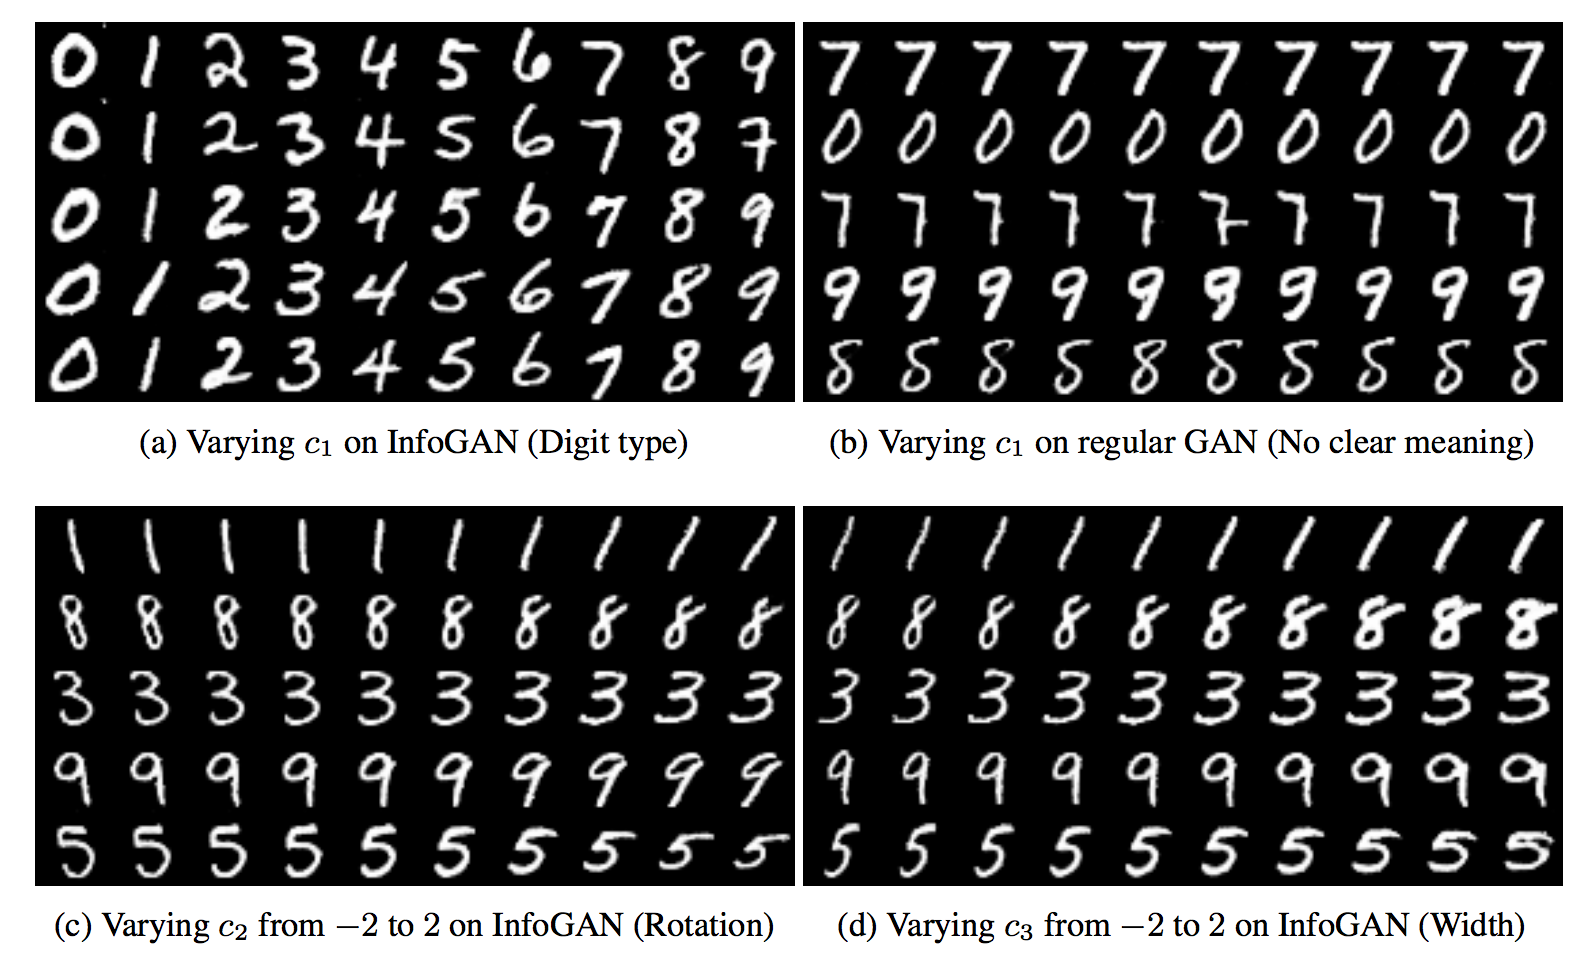
\includegraphics[width=\textwidth]{./img/17.png}
\caption{InfoGAN效果}
\label{fig:17}
\end{figure}
\subsection{调参技巧}
\subsubsection{Improved Techniques for Training GANs\cite{DBLP:journals/corr/SalimansGZCRC16}}
\subparagraph{Question}
GAN可以看成是找博弈的Nash equilibrium,但是并没有什么算法适合这种高维连续的参数空间。通过梯度下降不能保证博弈的收敛性,比如loss为xy,两边都会在正负两边循环而不能收敛到(0,0)。
文中介绍几个heuristic的方法缓解这个问题。
 \subparagraph{feature matching}
优化G只看结果偶然性较大,更精细一点是比较生成样本和真实样本在D中某个中间层的特征表示。令f为D到这个中间层的映射。
$$J^{(G)}=||\mathbb{E}_{x\sim data}f(x)-\mathbb{E}_{x\sim noise}f(G(x))||^2_2$$
 \subparagraph{Minibatch discrimination}
其实是一种层将$n\times A$的中间层映射为$n\times B$且将相互之间差异信息糅杂进去。
具体做法是用$A\times B \times C$的权值矩阵去乘,$out_{n,b}=\sum\limits_{i=1}^N e^{-||(in_iT)_b - (in_nT)_b||_1}$
事实证明这个不影响D的分类效果。
 \subparagraph{Historical averaging}
加正则与历史平均参数值的差$||\theta - \frac{1}{t}\sum \theta[i]||$。
 \subparagraph{One-sided label smoothing}
用0.1、0.9代替0、1。避免在截止区出现一系列问题。
 semi-supervised
K+1类,其中1类代表fake。分两段分别学习。
 \subparagraph{Inception Score}
$$e^{\mathbb{E}_xD_{KL}(p(y|x)||p(y))}$$
x为生成样本,y为类别。


\section{GAN应用}
\subsection{半监督学习}
\subsubsection{Semi-Supervised Learning with Generative Adversarial Networks\cite{DBLP:journals/corr/Odena16a}}
这是Improve GAN中提及的半监督学习的GAN的方式的出处,就是对于原来有分类的数据,将D的输入分成N+1类,这样可以同时做生成和判别两个任务。
效果主要在收敛效率上,这两个任务在初期或样本少的时候使用SGAN效果都比单独的Baseline要好。
\begin{figure}
\centering
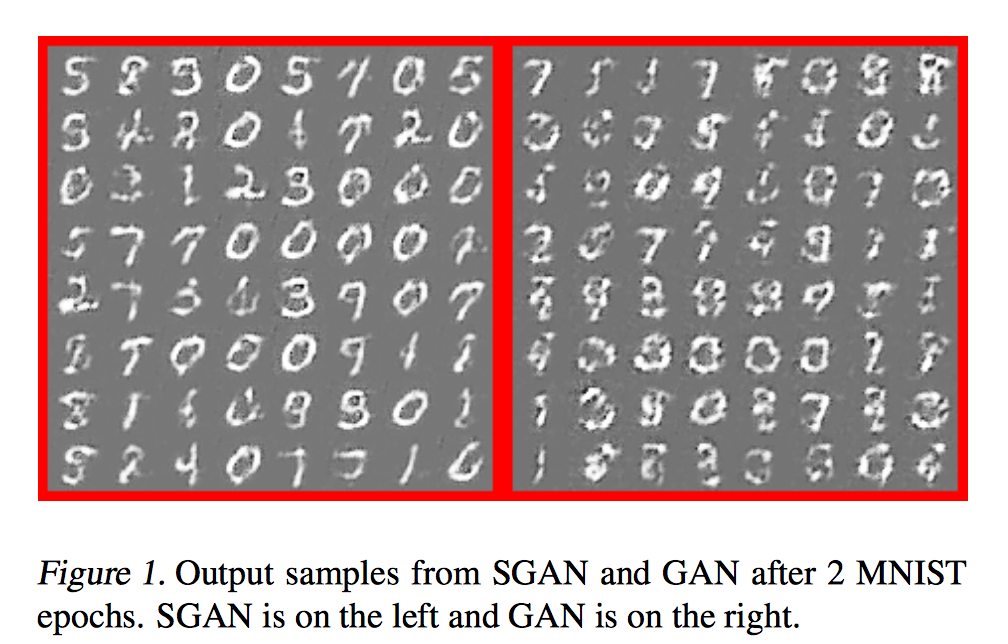
\includegraphics[width=\textwidth]{./img/20.png}
\caption{Semi-Supervised GAN效果}
\label{fig:20}
\end{figure}
\subsubsection{Triple Generative Adversarial Nets\cite{DBLP:journals/corr/LiXZZ17}}
这篇文章想同时解决两个问题:半监督的分类和已知种类标签的生成。

前者之前是通过增加判别器种类实现的,后者在AC-GAN中是通过classifier的loss实现的。

本文将generator、classifier、discriminator三者更紧密的结合在一起,判别器接受sample、label对判别是否真实,而这中sample、label对可能是真实sample+classifier生成的或者generator根据label生成的(本文中generator是conditional的)。最后加上真实数据和标签训练classifer的loss。
\begin{figure}
\centering
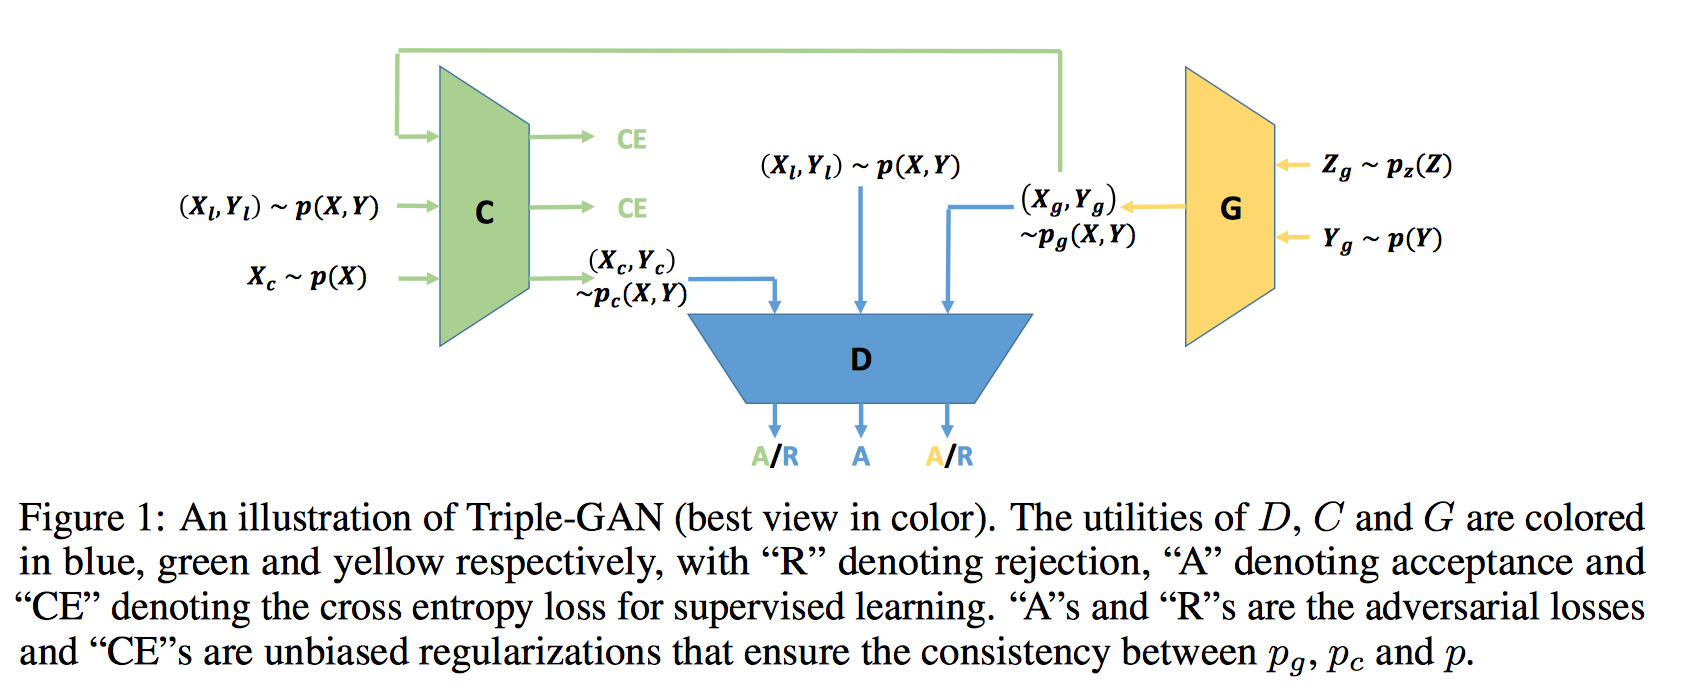
\includegraphics[width=\textwidth]{./img/32.png}
\caption{Triple GAN}
\label{fig:32}
\end{figure}
\begin{multline}
\min\limits_{C,G}\max\limits_D E_{(x,y)\sim p(x,y)}[\log D(x,y) - \log p_c(y|x)] +\\(1-\alpha)E_{y\sim p(y),z\sim p(z)}[\log(1-D(G(y,z), y))] + \alpha E_{x\sim p(x),y\sim p_c(y|x)}[\log (1 - D(x,y))]\nonumber
\end{multline}
\subsubsection{Good Semi-supervised Learning That Requires a Bad GAN\cite{DBLP:journals/corr/DaiYYCS17}}
kimi的一篇文章,他发现之前直接在D加入分成N类的方法理论上有很大问题。设想如果是完美的生成器,那么D将无法确定如何究竟应该分在K+1类还是生成的类别。事实上,GAN做半监督之所以有用是因为会生成一些真实分布不同mode之间的类别,从而让分类器将这些分辨开,使得这中间低密度区域两边的分类更加准确。
\begin{figure}
\centering
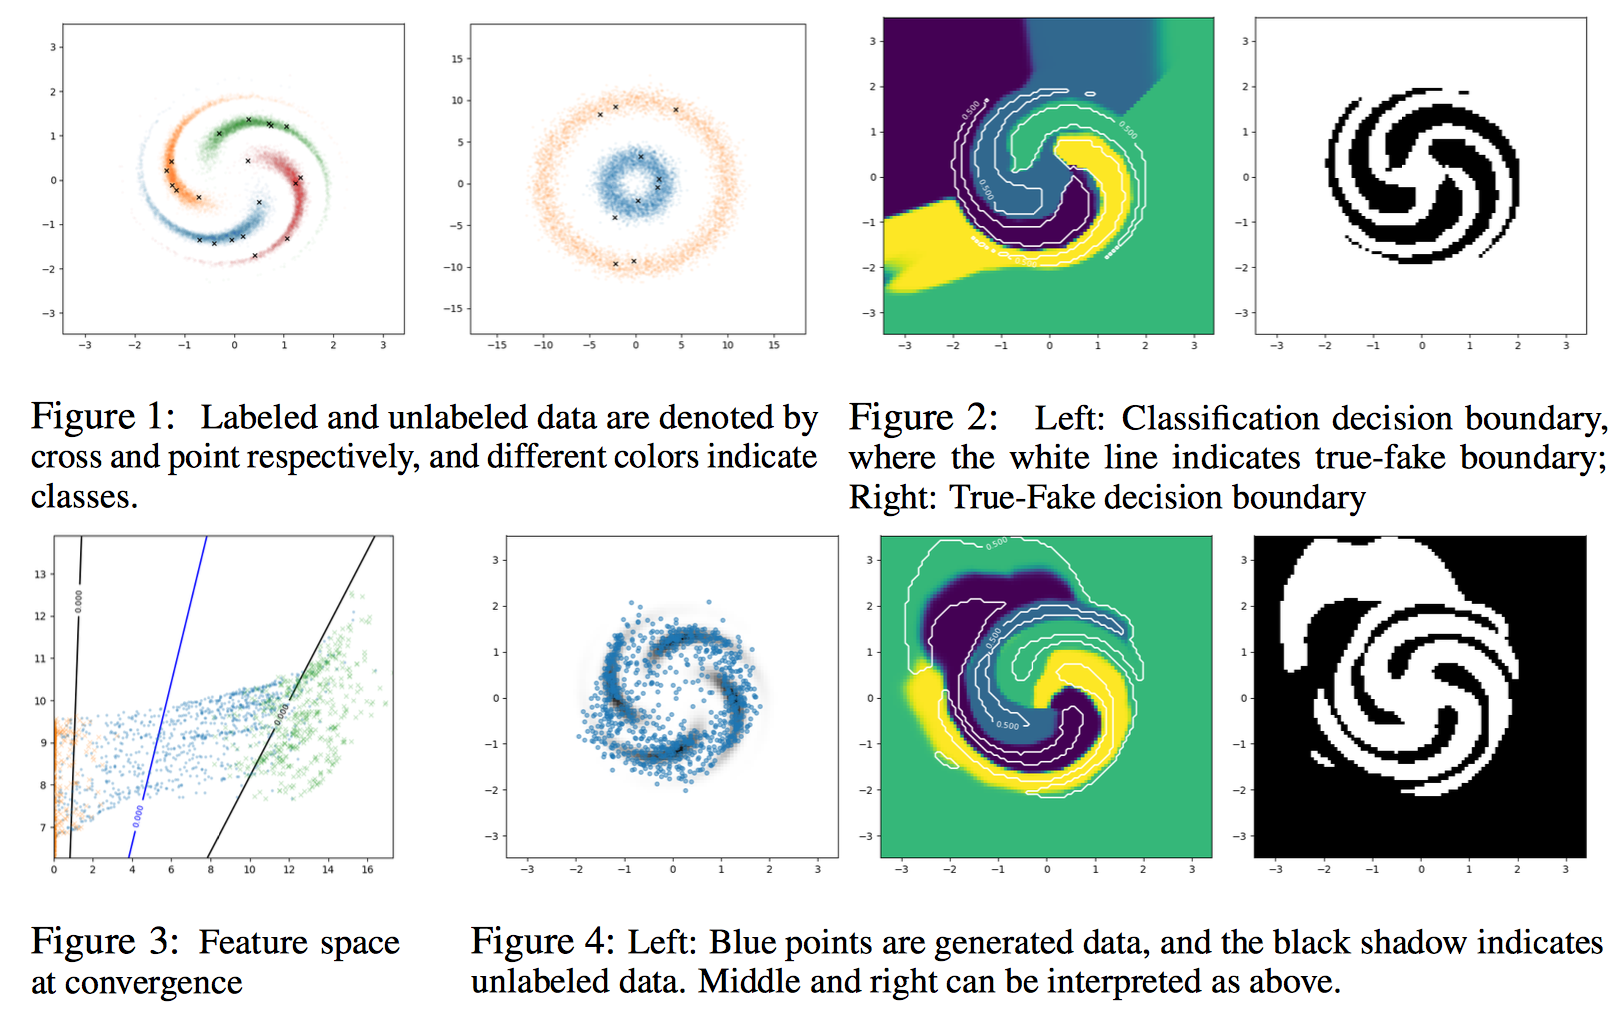
\includegraphics[width=\textwidth]{./img/33.png}
\caption{Semi-supervised GAN图解}
\label{fig:33}
\end{figure}
文章认为G产生的分布应该更接近于真实分布的补集,于是提出优化G与mode的凸集内概率为$\frac{1}{Z}\frac{1}{p(x)}$这个分布的KL散度,但为了保证其他地方没有分布,否则KL散度没法算,还得加上原来的loss。\ref{fig:33}

最后的loss是$$\min_G \quad -\mathcal{H}(p_G) + \mathbb{E}_{x \sim p_G} \log p(x) \mathbb{I}[p(x) > \epsilon]  + \|\mathbb{E}_{x \sim p_G} f(x) - \mathbb{E}_{x \sim \mathcal{U}} f(x)\|^2.
$$

第一项熵用类似与INFO GAN中的方法估计$-\mathcal{H}(p_G) \leq - \mathbb{E}_{x, z \sim p_G} \log q(z | x) = L_\text{VI}$,第二项用pixelCNN++\cite{DBLP:journals/corr/SalimansKCK17}的方法估计。
下面是判别器的损失函数,与之前类似,最后一项熵的意思是鼓励生成尖峰分布,使得判别出来的尽量靠近其中一个类。
\begin{equation}
\small
\begin{aligned}
\max_{D} \quad
& \mathbb{E}_{x, y \sim \mathcal{L}} \log p_D(y | x, y \leq K) + \mathbb{E}_{x \sim \mathcal{U}} \log p_D(y \leq K | x) + \\
& \mathbb{E}_{x \sim p_G} \log p_D(K + 1 | x)  + \mathbb{E}_{x \sim \mathcal{U}} \sum_{k = 1}^K p_D(k | x) \log p_D(k | x).
\label{eq:d_full}
\end{aligned}
\end{equation}
\subsection{Multi-View Image Generation from a Single-View\cite{DBLP:journals/corr/ZhaoWCLF17}}
这篇文章是通过conditional GAN框架做改动后,应用于已知一个角度图片,生成另一个角度图片的任务。
\begin{figure}
\centering
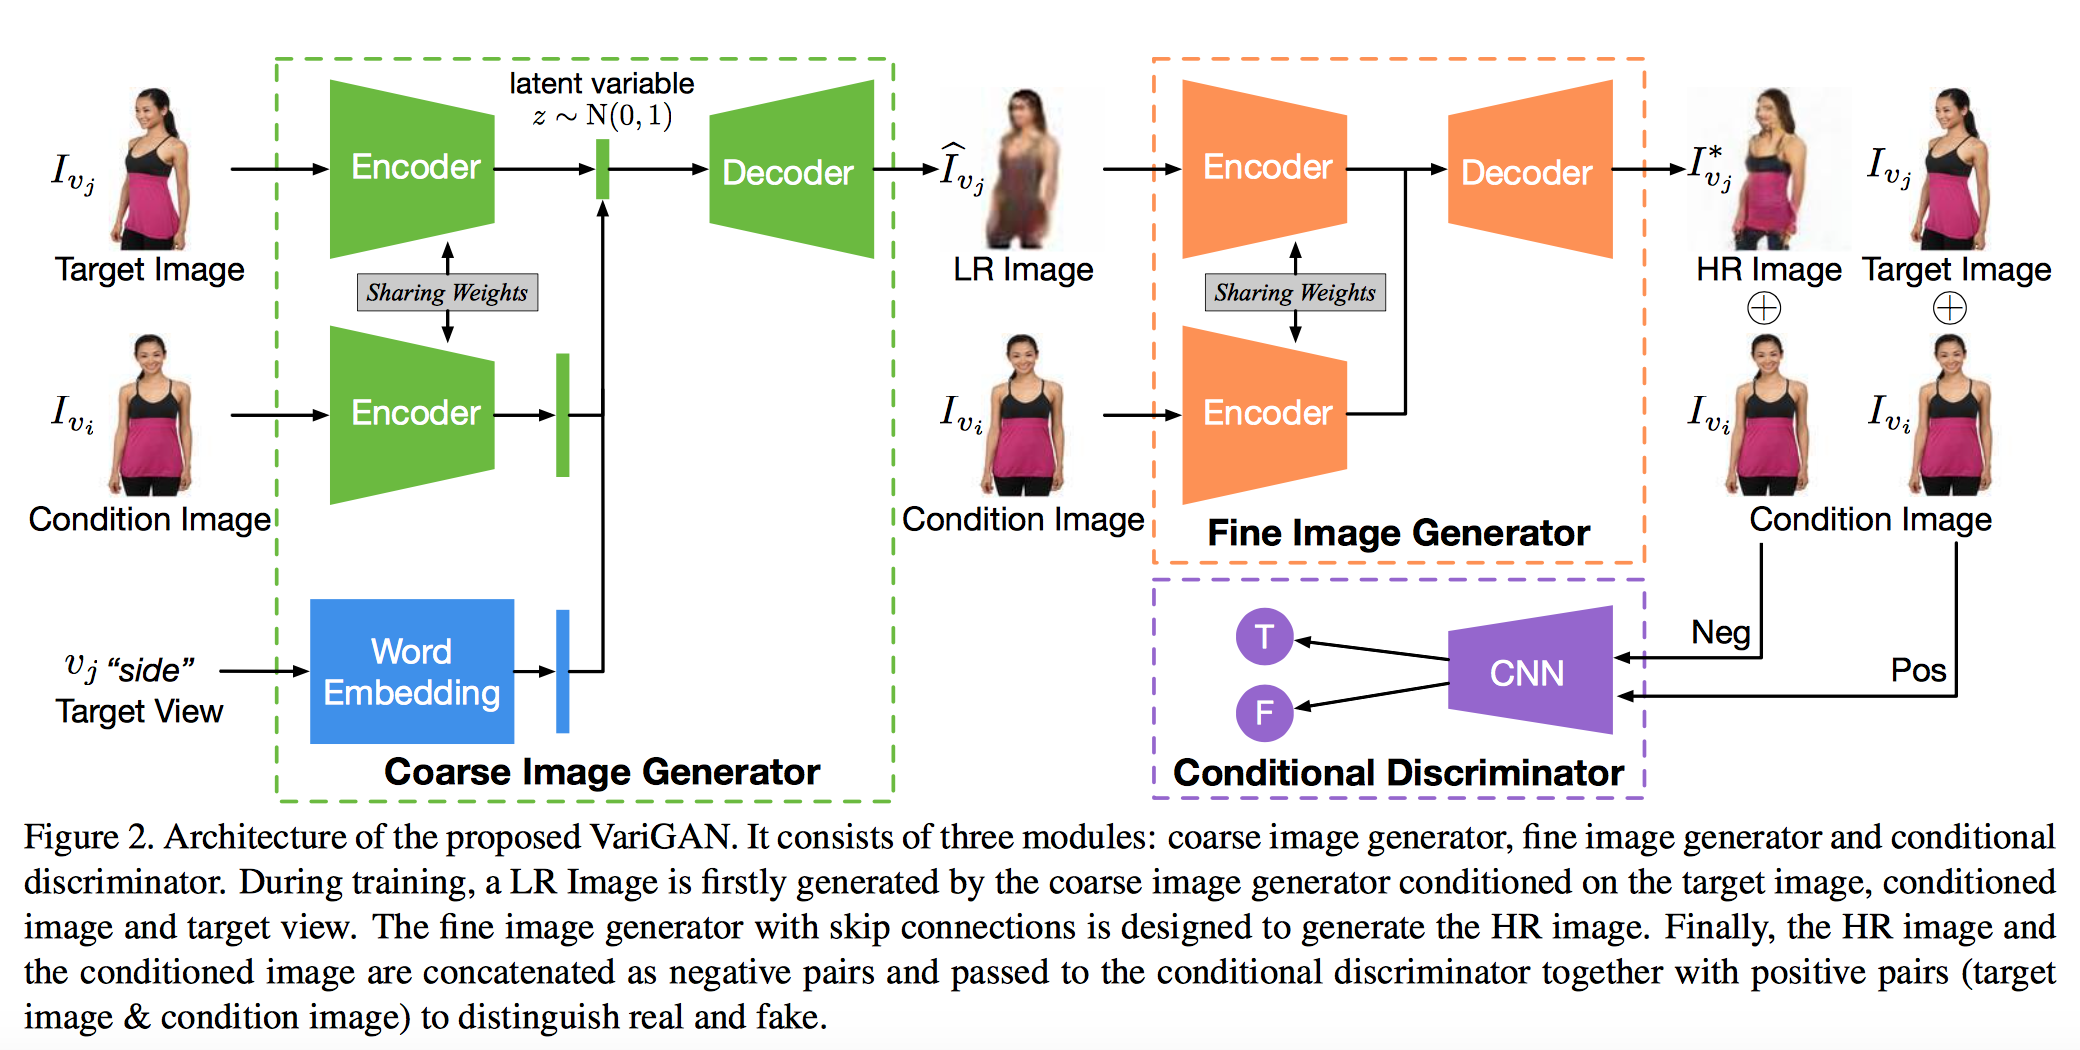
\includegraphics[width=\textwidth]{./img/39.png}
\caption{VariGAN架构}
\label{fig:39}
\end{figure}
首先生成一个模糊的框架,这里用到了变分的方法。之后将模糊框架和原图一起通过Conditional GAN生成另一个视角的图片\ref{fig:39},具体网络架构使用了UNet。

\subsection{Adversarial Training For Sketch Retrieval\cite{DBLP:journals/corr/CreswellB16}}
这篇应用文章使用GAN的角度很奇特,他使用了GAN来提取feature。普通的卷积网络可以提取feature,但监督学习的过程必须有label。GAN的D最后一层也可以认为是提取feature,但是是无监督的。

作者图像检索Merchant Marks,问题大概是这样的。
\begin{figure}
\centering
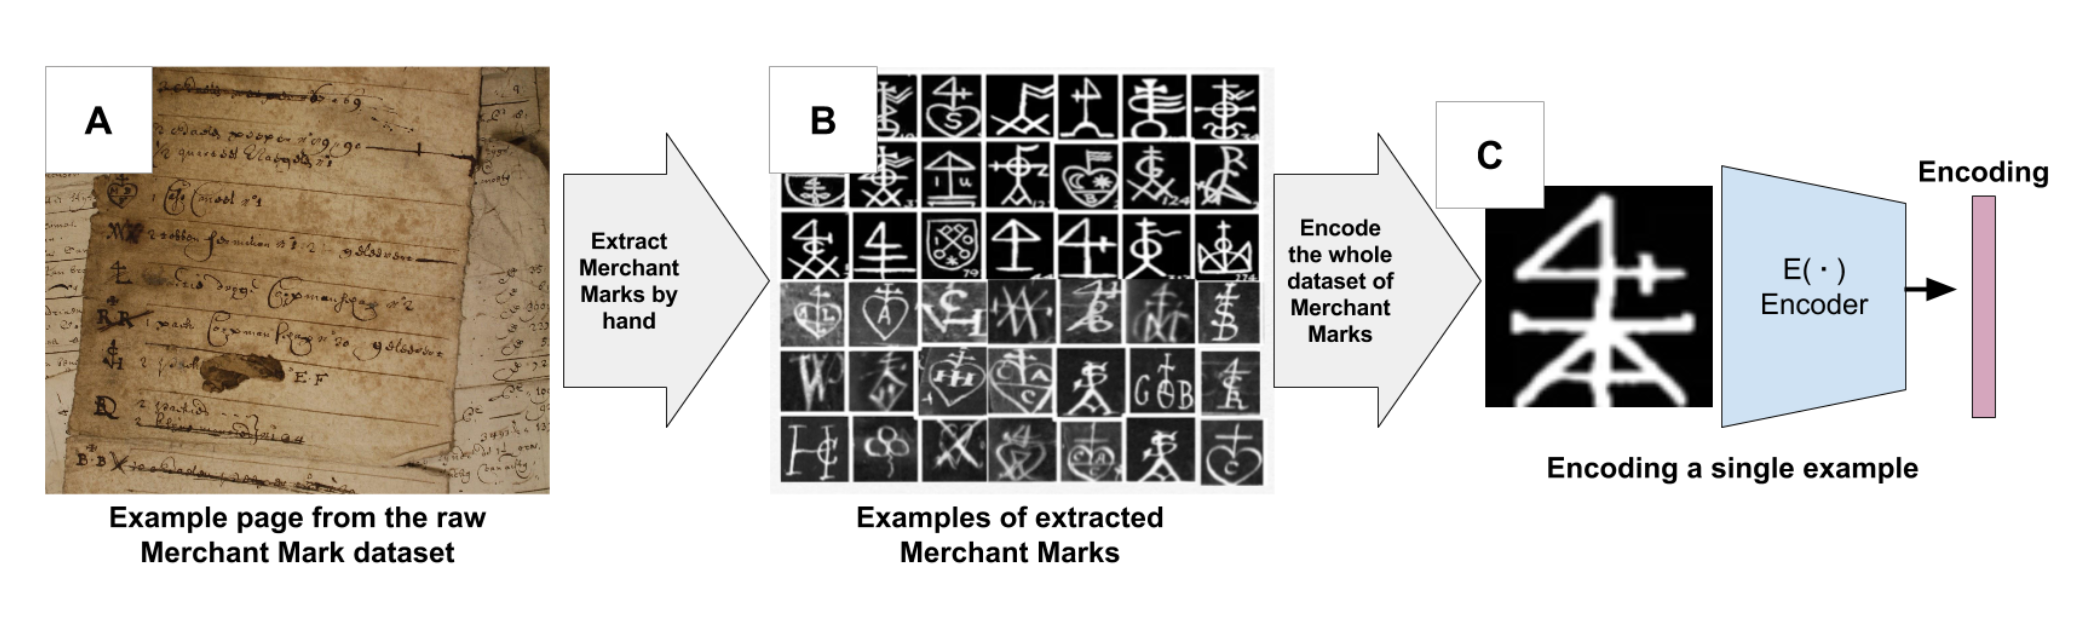
\includegraphics[width=\textwidth]{./img/22.png}
\caption{Sketch Retrieval问题简介}
\label{fig:22}
\end{figure}测试了两种普通的卷积神经网络框架,目测效果还不错。但是很奇怪没有定量地评价,也没有与其他提取feature的方法例如autoencoder等进行对比。
\subsection{Photo-Realistic Single Image Super-Resolution Using a Generative Adversarial Network\cite{DBLP:journals/corr/LedigTHCATTWS16}}
使用GAN提高图像的分辨率,就是用conditional GAN生成高分辨率图像。
loss分为3部分,一部分是跟原始图像的MSE,另一部分是GAN的loss,还有一个total variation正则项。
G和D都是层数不太多的ResNet。
\begin{figure}
\centering
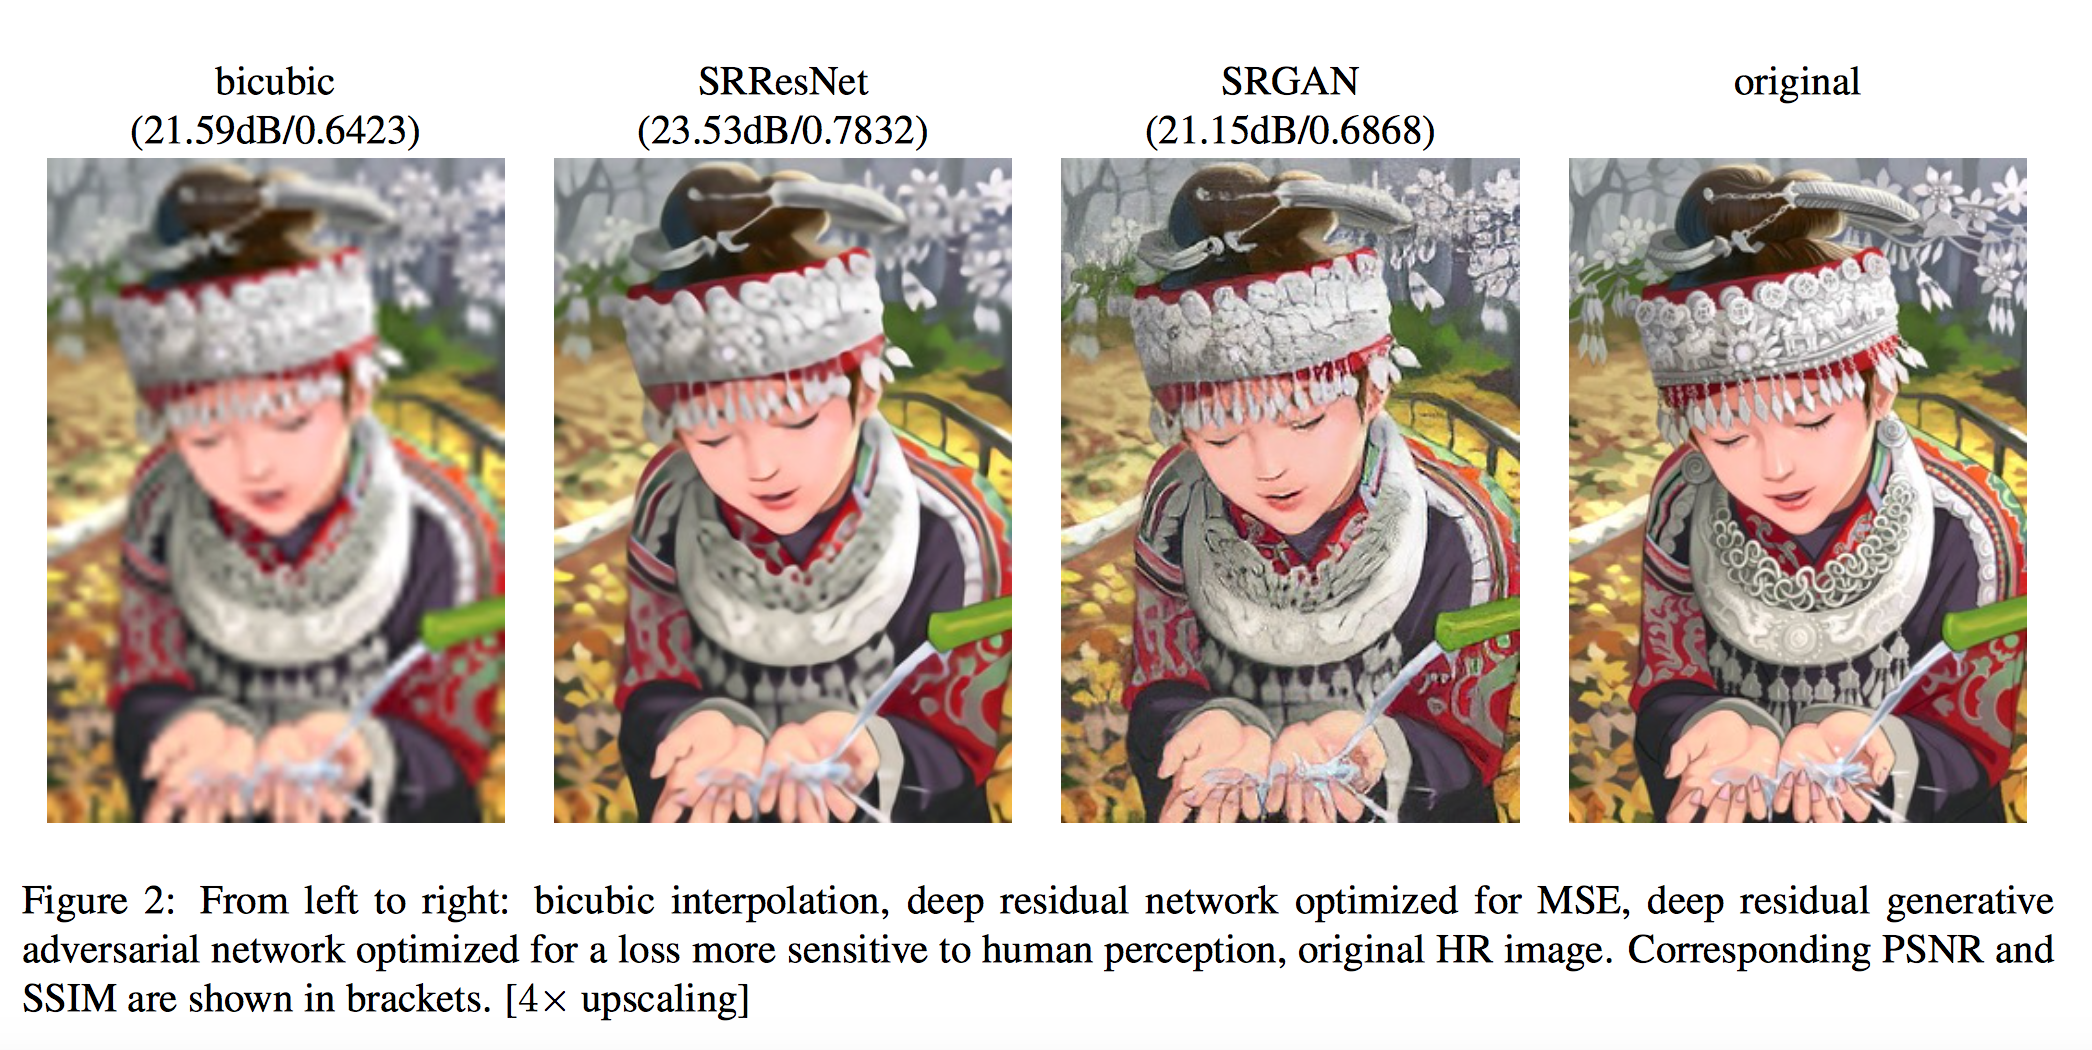
\includegraphics[width=0.8\textwidth]{./img/23.png}
\caption{SRGAN与其他方法}
\label{fig:23}
\end{figure}
PS:PSNR和SSIM都是越大越好。
这里谈的是第五版的论文,本次更新发现直接使用深度残差网络的SRResNet取得了最好的效果,但是作者认为目前这两种定量指标都不足以说明人类的感知评价,于是使用了主观评价指标MOS。确实感觉SRGAN得到的图片边缘比较锐利,人的主观评价得分比较高。
\subsection{SeqGAN: Sequence Generative Adversarial Nets with Policy Gradient\cite{DBLP:journals/corr/YuZWY16}}
\subparagraph{问题}
自然语言处理的序列生成的时候,使用GAN有两个问题:
\begin{itemize}
\item 离散样本问题,梯度没办法从D有效地传到G。
\item GAN只能对整个序列给定loss,不能对中间结果进行评价,使得训练的针对性不强。
\end{itemize}

\subparagraph{方法}
\begin{figure}
\centering
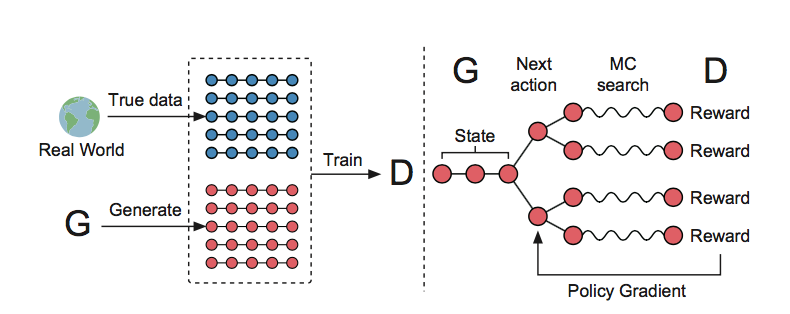
\includegraphics[width=\textwidth]{./img/24.png}
\caption{SeqGAN图解}
\label{fig:24}
\end{figure}解决问题的方法是用增强学习的policy gredient代替从D直接向G传的gredient。
定义$G_\theta(y_t|Y_{1:t-1})$为对于前面序列,生成下面\textbf{一个}元素的模型或policy。
设J为生成模型的reward,那么:
$$\nabla J(\theta)=\sum\limits_{y\in \mathcal{Y}}(\nabla G_\theta(y_t|Y_{1:t-1}))Q_{D_\phi}^{G_\beta}(Y_{1:t-1},y_t)$$
其中Y为某个$G_\theta$生成的样本,Q为回报估计函数:
$$Q_{D_\phi}^{G_\beta}(Y_{1:t-1},y_t)=\left\{
\begin{aligned}
D_\phi(Y_{1:t}),& if \ \ t=T\\
\frac{1}{N}\sum\limits^N_{n=1}D_\phi(Y_{1:T}^n), Y^n_{1:T} \in MC^{G_\beta}(Y_{1:t};N), & if \ \ t < N
\end{aligned}
\right.$$
也就是说,对于每一个自己生成的序列样本,只要D足够优秀,就可以计算生成模型在每一步生成元素的时候对应条件概率的梯度。这样一下子解决了上述两个问题:
\begin{itemize}

\item 离散样本没办法传梯度——原来loss function梯度的来源是$log(1-D(G(z,\theta)))$需要通过样本传,现在强化学习直接定义期望回报为$\sum_{y_1} G_\theta(y_1|s_0)\cdot Q_{D_\phi}^{G_\beta}(s_0, y_1)$是通过前面那部分传梯度的。
\item 只能衡量完整样本——但我每一步都通过蒙特卡洛补成完整样本再算reward
\end{itemize}
\begin{figure}
\centering
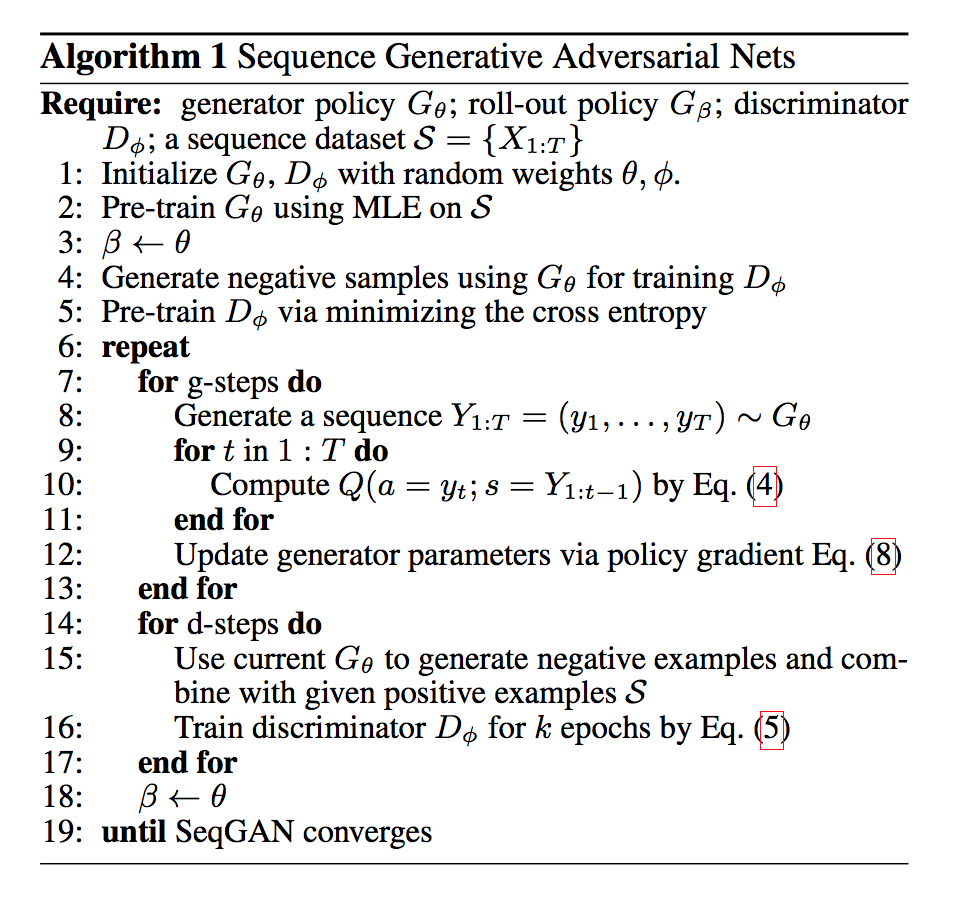
\includegraphics[width=0.8\textwidth]{./img/25.png}
\caption{SeqGAN算法描述}
\label{fig:25}
\end{figure}
(4)是上边的梯度公式,(5)是GAN的交叉熵,(8)是梯度下降。
\subsection{Style Transfer Generative Adversarial Networks: Learning to Play Chess Differently\cite{DBLP:journals/corr/ChidambaramQ17}}
\begin{figure}
\centering
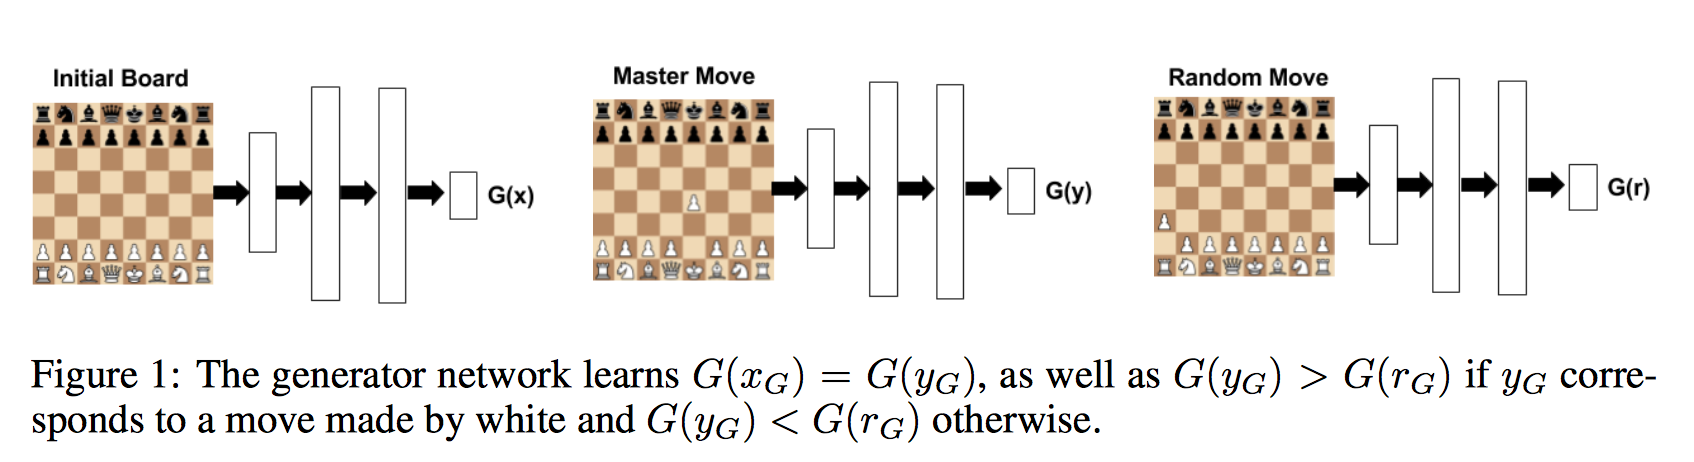
\includegraphics[width=\textwidth]{./img/40.png}
\caption{棋风变换}
\label{fig:40}
\end{figure}
这里的“风格”指的不是图像的风格,而是“棋风”,在某些情况下做出类似于某个人的下法。

毕竟是一篇应用的文章,想法很简单,就是conditional GAN,输入棋盘状态,输出下一步,然后判别是不是特定棋风的下法。\ref{fig:40}

但是由于真实样本不够,在某些情况出现的时候必须得到一个不错的下法,因此G加入另一个loss项,用log似然保证预测的下法尽量接近大师棋谱中的下法、远离随机下法。
\subsection{SEGAN: Speech Enhancement Generative Adversarial Network\cite{DBLP:journals/corr/PascualBS17}}
\begin{figure}
\centering
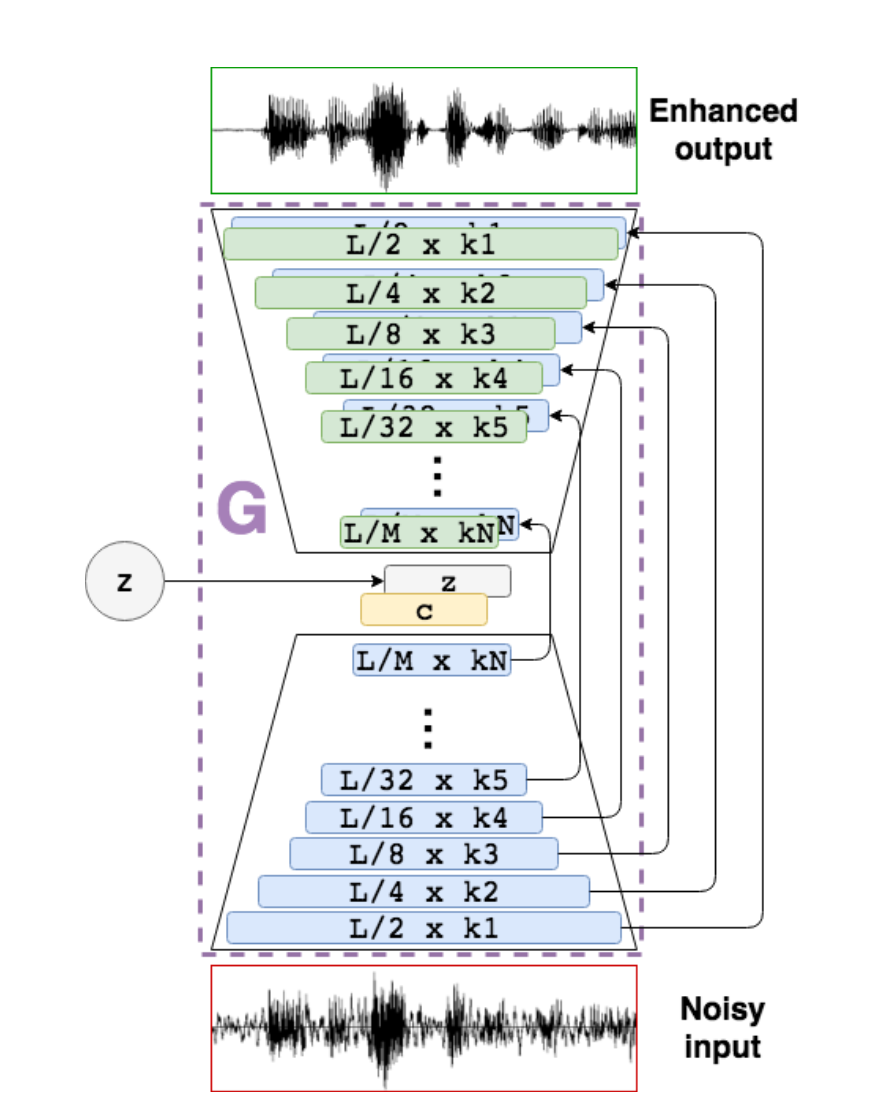
\includegraphics[width=\textwidth]{./img/43.png}
\caption{SEGAN生成网络结构}
\label{fig:43}
\end{figure}

\begin{figure}
\centering
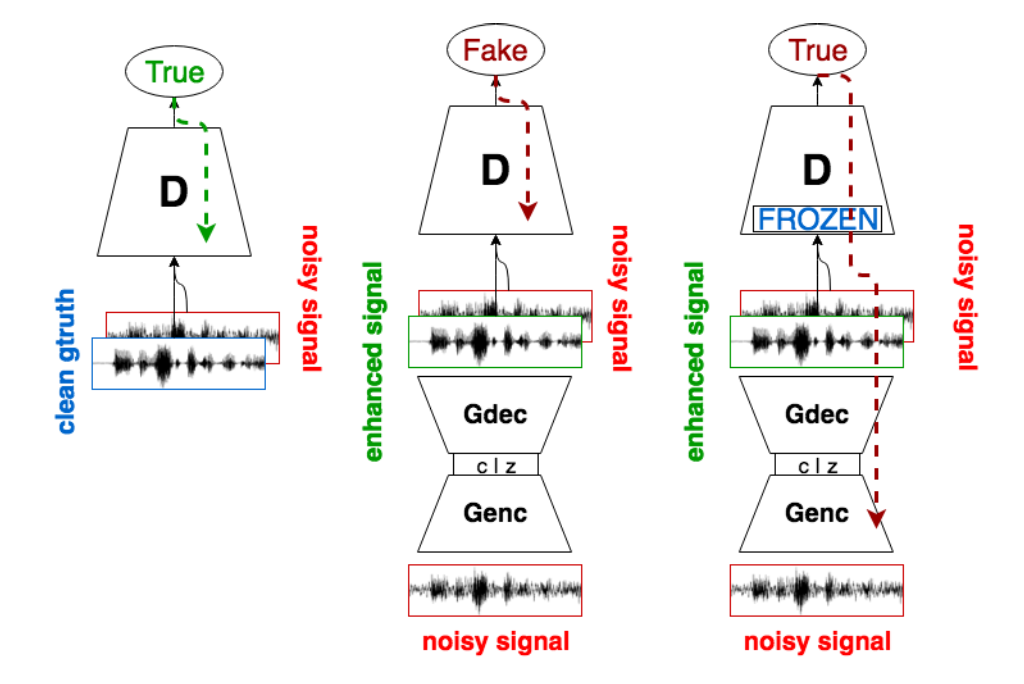
\includegraphics[width=\textwidth]{./img/42.png}
\caption{SEGAN整体网络结构}
\label{fig:42}
\end{figure}
这篇文章将GAN用于音频处理上,通过生成网络G除去噪音。对于信号的处理使用了一个encoder-decoder的结构,如\ref{fig:43}。

训练使用了Conditional GAN的方法,如\ref{fig:42}。
\section{强化学习}
\subsection{Playing Atari with Deep Reinforcement Learning\cite{DBLP:journals/corr/MnihKSGAWR13}}
\subparagraph{Question}
比起监督学习,强化学习有以下几个问题:

1. 没有很多的数据,只有一个sparse, noisy and delayed的环境。感觉环境提供的信息其实比数据更多,只是不容易处理。delay是最大的区别。
2. 监督学习要求样本独立,强化学习前后状态有明显相关性。如果将整个决策、状态序列当成一个样本,就是独立的。但是状态空间太大,需要使用马尔可夫过程MDP的假设,只与前面的有关。
3. 监督学习样本分布不变,而强化学习会随着你policy的更新而改变。这个应该是针对Q-learning等一类算法的,这里估计的长期reward依赖于某个policy,而这个reward会被拿来做学习的ground truth。

\subparagraph{Background}
optimal action-value function $$Q^*(s,a)=\max_\pi\mathbb{E}[R_t|s_t=s,a_t=a,\pi]$$

其中$R_t$为未来折扣回报$R_t=\sum \gamma^{t'-t}r_{t'}$
Bellman equation $$Q^*(s, a) = \mathbb{E}_{s'\sim \varepsilon}[r_{t+1} + \gamma\max\limits_{a'}Q^* (s',a')|s,a]$$
于是在把s看做序列的情况下可以计算,但状态量恐怖。

使用机器学习的思想,确定F(s),如果状态空间很大,不同状态的取值有一定相关性,那么参数化为$f(s,\theta)$

于是$$L(\theta_i) = \mathbb{E}_{s,a\sim \rho(\cdot)}(y_i - Q(s,a,\theta_i)), y_i = \mathbb{E}_{s'\sim \varepsilon}[r_{t+1} + \gamma\max\limits_{a'}Q^(s',a')|s,a]$$

\subparagraph{Method}

\begin{figure}
\centering
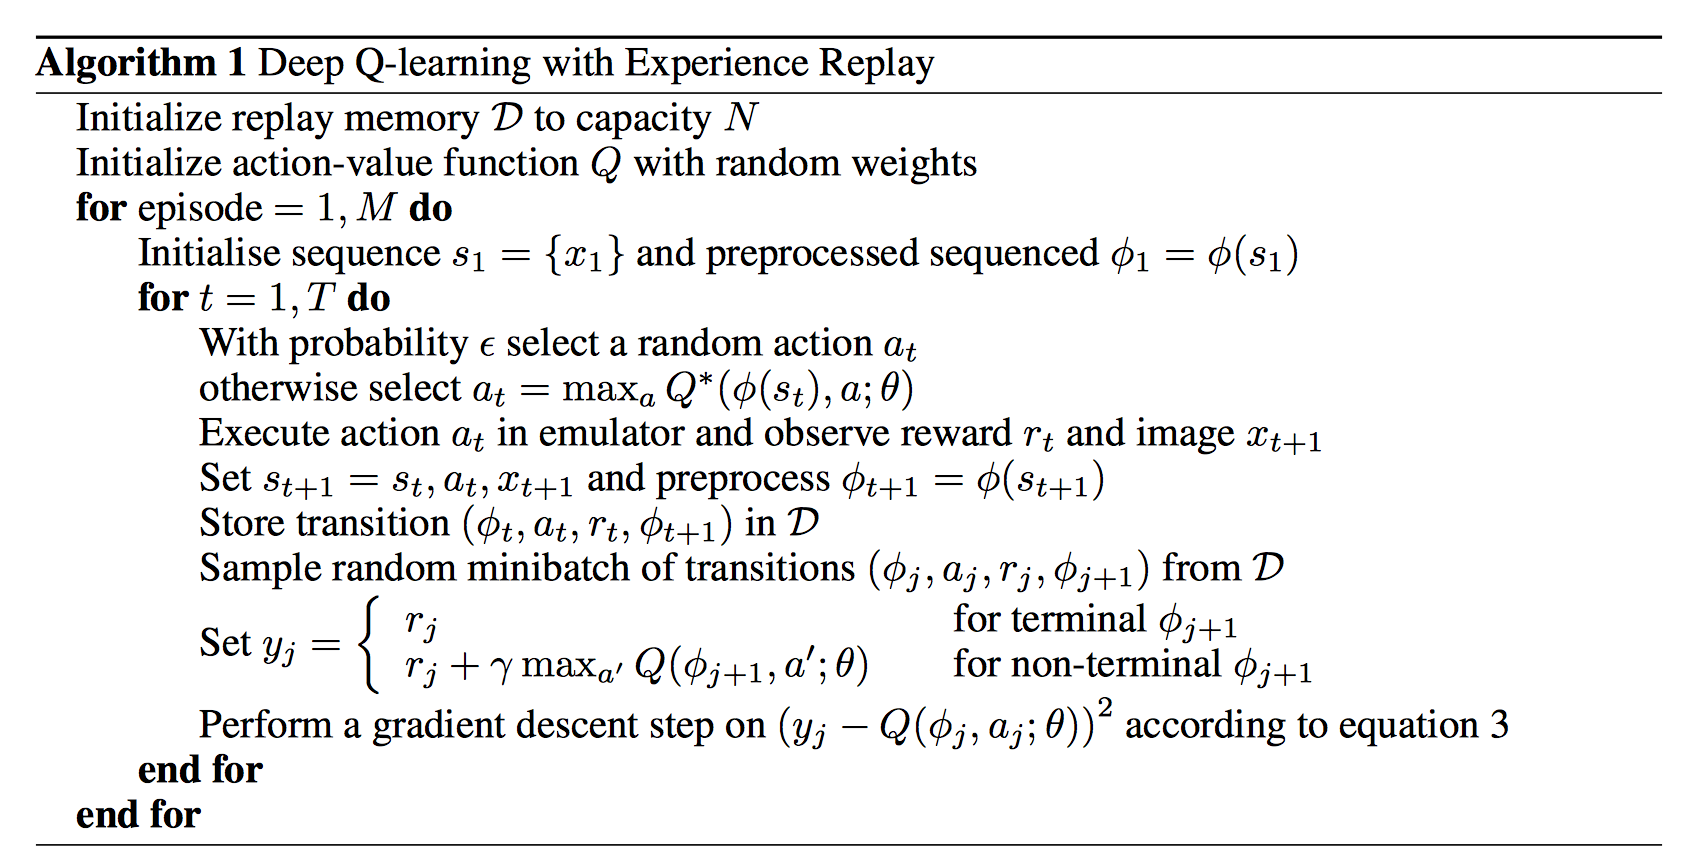
\includegraphics[width=0.8\textwidth]{./img/26.png}
\caption{DQN算法描述}
\label{fig:26}
\end{figure}
这里改进的主要是采样方法使用了$\varepsilon-greedy$和每次随机更新之前采取过的transition。这样想当于一个smooth的过程,才可能收敛。

Q的输入有$\phi(s)、a$,二者很难直接并列输入,最后采取了根据不同a设置不同的最后一层的方法。

可能是由于决策的局部性,如果更新当前的transition的话容易被某种连续的策略dominate。
\subsection{Human-level control through deep reinforcement learning\cite{Mnih2015Human}}
这是上一篇文章之后DeepMind发表在Nature上的一个改进版本。最重要的改进是把原来计算ground truth时的使用$Q(\phi_{j+1},a';\theta)$改为一个参数更新有延迟版本的网络,更好地解决原来那个训练不稳定的问题。
\begin{figure}
\centering
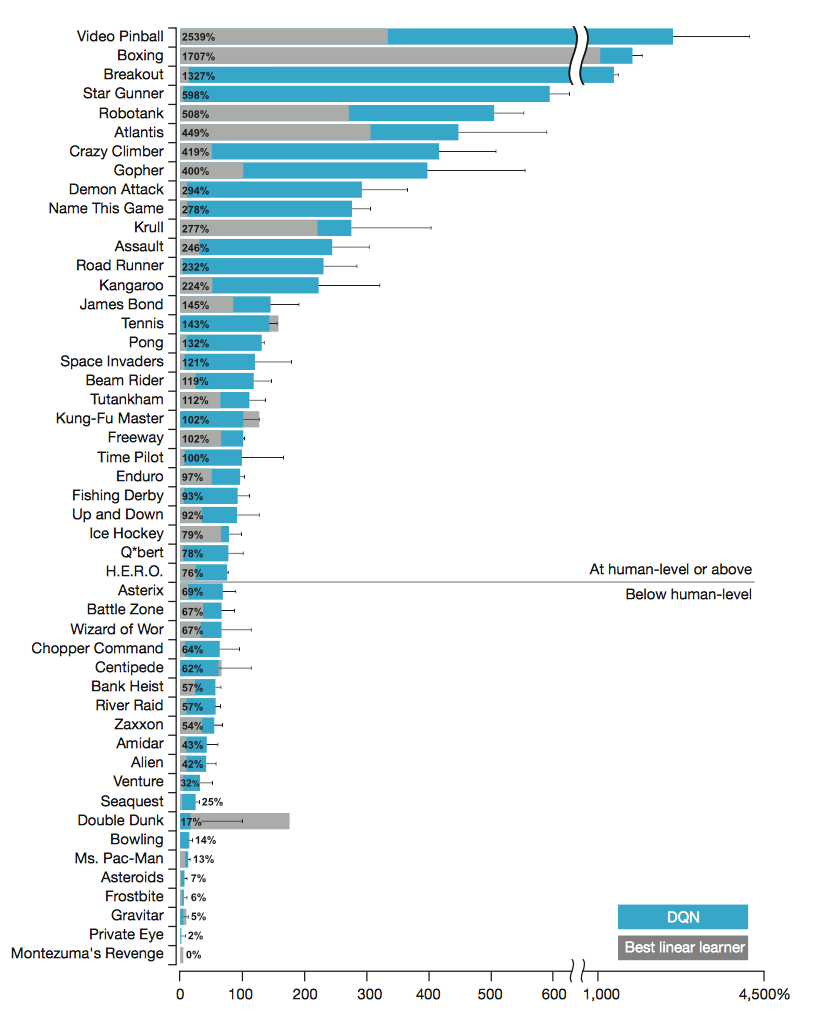
\includegraphics[width=0.8\textwidth]{./img/27.png}
\caption{DQN游戏水平}
\label{fig:27}
\end{figure}
另外做了详细的测试\ref{fig:27}。
\subsection{Deep Reinforcement Learning with Double Q-learning\cite{DBLP:journals/corr/HasseltGS15}}
针对目标函数y是max得到的对结果有偏这个问题做出改进。
首先$m \ estimates \ x,\sum x - x_{real} = 0, \sum (x-x_{real})^2=mC$
可以证明$$\max x_i \geq x_{real} + \sqrt{\frac{C}{m-1}}$$

证明很容易,首先分成偏差为正负两类,每类和一定,使得方差最大显然要一个为和,其他为0。但是正的最大不得超过$\sqrt{\frac{C}{m-1}}$(反证),所以最后取最优就在m-1个正的$\sqrt{\frac{C}{m-1}}$$,一个$$-(m-1)\sqrt{\frac{C}{m-1}}$

(感觉不太符合题意,毕竟并不是每个action都是最优action的无偏估计,但是道理是这样的)

如何解决,将Nature DQN target network选取最大的是按照select network选取的……反正效果不错。
\begin{figure}
\centering
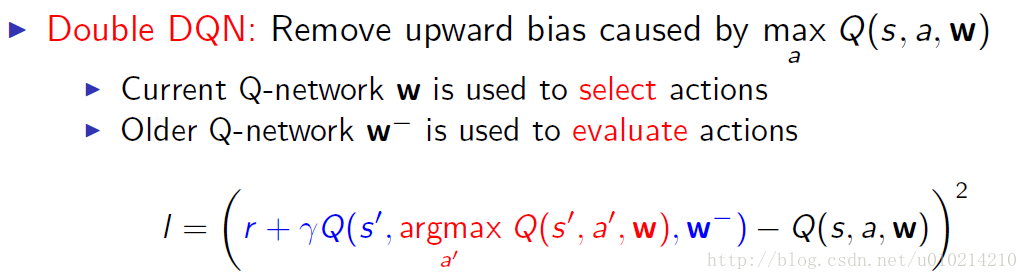
\includegraphics[width=0.8\textwidth]{./img/28.png}
\caption{Double-DQN}
\label{fig:28}
\end{figure}

\subsection{Dueling Network Architectures for Deep Reinforcement Learning\cite{DBLP:journals/corr/WangFL15}}
\subparagraph{Question}
之前处理s和action输入关系的时候,对每个action确定一个输出层,这样不自然。
\subparagraph{Method}
\begin{figure}
\centering
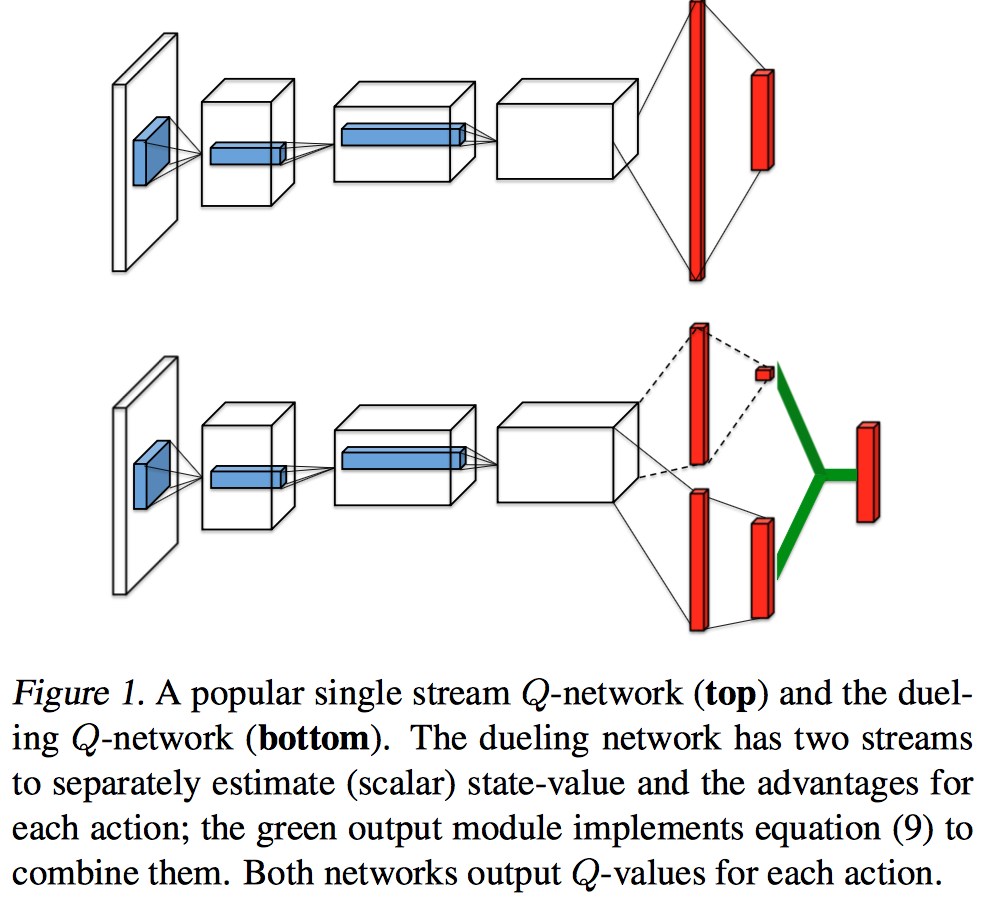
\includegraphics[width=0.8\textwidth]{./img/29.png}
\caption{Dueling DQN图解}
\label{fig:29}
\end{figure}将输入图像经过卷积处理之后,分成两部分,一部分计算出当前这个状态的价值,另一部分计算执行action的价值。
$$Q(s,a;\theta,\alpha,\beta)=V(s,\theta, \alpha) + A(s,a,\beta)$$
注意要归一,否则两部分相对规模不能确定。
$$Q(s,a;\theta,\alpha,\beta)=V(s,\theta, \alpha) + (A(s,a,\beta) - \max A(s,a,\beta))$$减去最大值也可换成平均值。


\bibliographystyle{plainnat}
\bibliography{sample}

\end{document}